\documentclass[letterpaper,journal]{IEEEtran}
\usepackage{amsmath,amsfonts}
\usepackage{algorithmic}
\usepackage{algorithm}
\usepackage{array}
\usepackage[caption=false,font=normalsize,labelfont=sf,textfont=sf]{subfig}
\usepackage{textcomp}
\usepackage{stfloats}
\usepackage{url}
\usepackage{verbatim}
\usepackage{graphicx}
\usepackage{cite}

\hyphenation{op-tical net-works semi-conduc-tor IEEE-Xplore}

\begin{document}

% 正式英文论文标题。
\title{Towed Movable Antenna-Assisted Near-Field Integrated\\ Sensing and Communication}

% 作者、单位等
\author{Author Name}

\maketitle

\begin{abstract}
% 在这里填写英文摘要。
Your abstract goes here.
\end{abstract}

\begin{IEEEkeywords}
% 这里填写 3--6 个关键词。
Towed movable antenna (ToMA), integrated sensing and communication (ISAC), near-field, full-duplex, antenna position optimization.
\end{IEEEkeywords}

% ============================================================
% 第一节 Introduction。
% 你完成英文引言后，直接替换下面这一段占位文字。
% ============================================================
\section{Introduction}

The main contributions of this paper are summarized as follows:
\begin{enumerate}
    \item \textbf{ToMA-assisted full-duplex near-field ISAC modeling and joint problem formulation:}
    We consider a full-duplex near-field ISAC system consisting of a main UAV and multiple towed sub-UAVs. The transmit and receive ToMA arrays are reconfigured in three-dimensional space through fixed-length cables, with the antenna elements on each cable moving in a coupled manner as its endpoint changes. Near-field spherical-wave models are adopted for the communication and sensing channels, while the two-way target-echo attenuation and geometry-dependent residual self-interference are taken into account. Subject to fixed cable lengths, inter-UAV collision-avoidance constraints, and transmit-power limits, we formulate a weighted sum-rate (WSR) maximization problem that jointly optimizes the ToMA geometry, transmit beamformers, UL transmit powers, and UL communication and sensing receive beamformers.

    \item \textbf{Two-layer alternating optimization integrating FP and FP-aware RCG:}
    To tackle the formulated nonconvex problem, we develop a two-layer alternating optimization framework comprising inner-layer resource optimization and outer-layer ToMA geometry optimization. In the inner layer, the Lagrangian dual transform (LDT) and quadratic transform (QT) are employed to handle the nonconvex fractional structure of the communication and sensing rate expressions. The transmit beamformers, UL transmit amplitudes, and UL communication and sensing receive beamformers are then updated alternately. In the outer layer, Riemannian conjugate gradient (RCG) optimization on spherical manifolds is used to update the cable-constrained ToMA endpoints. In particular, to alleviate the mismatch between a candidate geometry and the current resource allocation, an FP-aware candidate-evaluation mechanism is incorporated into the position search. Each candidate geometry is evaluated after a limited number of warm-start FP resource updates, and the updated geometry and resource state are accepted jointly according to an Armijo-type criterion. Multiple initializations are further employed to mitigate sensitivity to the initial solution.

    \item \textbf{Numerical evaluation under various benchmarks and system conditions:}
    We compare the proposed method with benchmark schemes based on fixed ToMA arrays, fixed uniform planar arrays (UPAs), and conventional independently movable antennas (MAs). The proposed method is evaluated in terms of convergence behavior, maximum DL transmit power, residual self-interference, system load, and the communication--sensing trade-off. Numerical results show that the proposed scheme achieves favorable WSR performance under the considered scenarios and parameter settings. In particular, it attains the highest numerical WSR among the four FP-based schemes at all 20 tested communication-weight values in the trade-off experiment. These results indicate that joint ToMA geometry reconfiguration and communication--sensing resource optimization can achieve competitive system performance despite the cable-coupled movement constraints.
\end{enumerate}

\section{System Model and Problem Formulation}
\label{sec:system_model}

Consider a ToMA-aided full-duplex near-field integrated sensing and communication (ISAC) system. The main UAV serves as the central platform for communication and sensing and is assumed to hover at a fixed location. It tows multiple UAVs through $M$ fixed-length cables to form reconfigurable transmit and receive arrays. All cables are attached to a common anchor point on the main UAV, where half of the towing UAVs constitute the transmit ToMA array and the remaining half constitute the receive ToMA array. Over the same time-frequency resource, the transmit ToMA array simultaneously communicates with $K$ downlink (DL) users and illuminates $L$ sensing targets, while the receive ToMA array simultaneously receives communication signals from $J$ uplink (UL) users and reflected echoes from multiple sensing targets. In this paper, the trajectory, global translation, and attitude of the main UAV are not optimized. Instead, the system performance is enhanced by jointly optimizing the ToMA geometry and the communication and sensing resources.

Unlike conventional fixed-position antenna (FPA) arrays and movable antenna (MA) architectures in which individual antenna elements can move independently, the ToMA array reconfigures its geometry by adjusting the positions of the towing UAVs, such that multiple antenna elements mounted on the same cable move in a coupled manner. Since the array aperture of the ToMA varies with the towing-UAV positions, the near-field operating region is determined according to the actual apertures of the transmit and receive ToMA arrays. Let $D_{\rm T}$ and $D_{\rm R}$ denote the effective apertures of the transmit and receive ToMA arrays, respectively. For $x\in\{{\rm T},{\rm R}\}$, the corresponding radiative near-field region can be approximately characterized as $0.62\sqrt{D_x^3/\lambda}<r<2D_x^2/\lambda$, where $\lambda$ denotes the carrier wavelength. In this paper, the communication users and sensing targets are considered to lie within the radiative near-field region of the ToMA arrays. Accordingly, spherical-wave channel models are adopted for the communication and sensing links.

Moreover, to account for the self-interference (SI) caused by simultaneous transmission and reception in the full-duplex mode, we adopt a unified equivalent residual self-interference (RSI) model. Specifically, the aggregate residual effect after passive isolation, analog cancellation, and digital cancellation is represented by $\mathbf H_{\rm RSI}$. The RSI is not imposed as an additional feasibility constraint; instead, it affects the system weighted sum rate (WSR) through the SINRs of the UL communication and sensing links.

% 中文注释：A. ToMA 几何模型
\subsection{ToMA Geometry Model}
\label{subsec:toma_geometry}

To describe the three-dimensional (3D) geometry of the ToMA arrays, we establish a global 3D Cartesian coordinate system $O\!-\!xyz$ centered at the main UAV, with the common cable anchor point coinciding with the origin, i.e., $\mathbf q_0=\mathbf o=\mathbf 0$. Let the sets of DL users, UL users, and sensing targets be $\mathcal K=\{1,\ldots,K\}$, $\mathcal J=\{1,\ldots,J\}$, and $\mathcal L=\{1,\ldots,L\}$, respectively. Their 3D coordinates are denoted by $\mathbf q_k^{\rm D}$, $\mathbf q_j^{\rm U}$, and $\mathbf q_l^{\rm S}\in\mathbb R^3$, where $k\in\mathcal K$, $j\in\mathcal J$, and $l\in\mathcal L$.

The system contains $M$ towing UAVs, where $M$ is assumed to be even. Define the towing-UAV index set as $\mathcal M=\{1,\ldots,M\}$. The first $M/2$ UAVs form the transmit ToMA array, while the remaining $M/2$ UAVs form the receive ToMA array, i.e., $\mathcal M_{\rm T}=\{1,\ldots,M/2\}$ and $\mathcal M_{\rm R}=\{M/2+1,\ldots,M\}$. The transmit/receive role of each towing UAV remains fixed within one optimization interval. Each cable carries $N_{\rm c}$ uniformly distributed antenna elements. Hence, the transmit and receive arrays each contain $N_{\rm T}=N_{\rm R}=MN_{\rm c}/2$ antenna elements.

Let $\mathbf c_m\in\mathbb R^3$ denote the endpoint position of the $m$-th towing UAV relative to the main UAV. Since the antenna elements are uniformly distributed along the $m$-th cable, the position of its $n$-th antenna element is given by
\begin{equation}
\mathbf p_{m,n}
=
\frac{n}{N_{\rm c}}\mathbf c_m,
\qquad
n=1,\ldots,N_{\rm c}.
\label{eq:cable_element_position}
\end{equation}
Therefore, all antenna-element positions on the same cable are jointly determined by the corresponding endpoint $\mathbf c_m$.

For a transmit cable $m\in\mathcal M_{\rm T}$, define the global transmit-antenna index as $i=(m-1)N_{\rm c}+n$, and let $\mathbf p_i^{\rm T}:=\mathbf p_{m,n}$, $i=1,\ldots,N_{\rm T}$. Similarly, for a receive cable $m\in\mathcal M_{\rm R}$, define the global receive-antenna index as $s=\left(m-\frac{M}{2}-1\right)N_{\rm c}+n$, and let $\mathbf p_s^{\rm R}:=\mathbf p_{m,n}$, $s=1,\ldots,N_{\rm R}$.

The endpoint positions associated with the transmit and receive ToMA arrays are stacked as $\widetilde{\mathbf c}_{\rm T}=\left[\mathbf c_m^T\right]_{m\in\mathcal M_{\rm T}}^T$ and $\widetilde{\mathbf c}_{\rm R}=\left[\mathbf c_m^T\right]_{m\in\mathcal M_{\rm R}}^T$, respectively. The joint ToMA endpoint-position vector is further defined as $\widetilde{\mathbf c}=[\widetilde{\mathbf c}_{\rm T}^T,\widetilde{\mathbf c}_{\rm R}^T]^T$. Since the communication, sensing, and SI channels all vary with these endpoint positions, $\widetilde{\mathbf c}$ constitutes the key geometric optimization variable of the proposed ToMA system.

Since all cables have a fixed length $L_{\rm c}$, the endpoint of each towing UAV must satisfy
\begin{equation}
\|\mathbf c_m\|_2
=
L_{\rm c},
\qquad
\forall m\in\mathcal M.
\label{eq:cable_length_constraint}
\end{equation}
In addition, to avoid collisions among the towing UAVs, the endpoint positions are constrained by
\begin{equation}
\|\mathbf c_m-\mathbf c_{m'}\|_2
\ge
D_{\rm UAV},
\qquad
\forall m\neq m'.
\label{eq:uav_distance_constraint}
\end{equation}
Thus, each towing UAV is constrained to move on a sphere centered at the main UAV with radius $L_{\rm c}$, while also satisfying the minimum inter-UAV safety-distance requirement.

% B. 近场信道模型
\subsection{Near-Field Channel Model}
\label{subsec:channel_model}

We consider a quasi-static narrowband line-of-sight (LoS) propagation environment and adopt the uniform spherical wave (USW) model for the communication, sensing, and SI channels. Unlike the conventional far-field plane-wave model, the near-field spherical-wave model preserves the actual propagation distance between each antenna element and each user or target, thereby capturing the phase variations induced by ToMA geometry reconfiguration. Let $\lambda$ denote the carrier wavelength and define the wavenumber as $k_0=2\pi/\lambda$. For an arbitrary spatial position $\mathbf q$, the near-field array response vectors of the transmit and receive ToMA arrays are respectively defined as
\begin{equation}
\mathbf a_{\rm T}
(\widetilde{\mathbf c}_{\rm T},\mathbf q)
=
\left[
e^{j k_0\|\mathbf p_i^{\rm T}-\mathbf q\|_2}
\right]_{i=1}^{N_{\rm T}},
\label{eq:tx_nf_response}
\end{equation}
and
\begin{equation}
\mathbf a_{\rm R}
(\widetilde{\mathbf c}_{\rm R},\mathbf q)
=
\left[
e^{j k_0\|\mathbf p_s^{\rm R}-\mathbf q\|_2}
\right]_{s=1}^{N_{\rm R}}.
\label{eq:rx_nf_response}
\end{equation}
Here, $\|\mathbf p_i^{\rm T}-\mathbf q\|_2$ and $\|\mathbf p_s^{\rm R}-\mathbf q\|_2$ represent the actual propagation distances from the $i$-th transmit antenna and the $s$-th receive antenna to position $\mathbf q$, respectively. Therefore, changing the towing-UAV endpoint positions alters the antenna coordinates and, consequently, the spherical-wave phase responses of the corresponding links.

Let $r_k^{\rm D}=\|\mathbf q_k^{\rm D}\|_2$ and
$r_j^{\rm U}=\|\mathbf q_j^{\rm U}\|_2$ denote the reference
propagation distances from the common anchor point at the main UAV
to DL user $k$ and UL user $j$, respectively. Under free-space LoS
propagation, the corresponding common amplitude path gains are modeled
as $\alpha_k^{\rm D}=\lambda/(4\pi r_k^{\rm D})$ and
$\alpha_j^{\rm U}=\lambda/(4\pi r_j^{\rm U})$, respectively.

Accordingly, the DL channel of user $k$ is expressed as
\begin{equation}
\mathbf h_k
=
\alpha_k^{\rm D}
\mathbf a_{\rm T}
(\widetilde{\mathbf c}_{\rm T},\mathbf q_k^{\rm D}),
\qquad
k\in\mathcal K,
\label{eq:dl_channel}
\end{equation}
while the UL channel of user $j$ is
\begin{equation}
\mathbf f_j
=
\alpha_j^{\rm U}
\mathbf a_{\rm R}
(\widetilde{\mathbf c}_{\rm R},\mathbf q_j^{\rm U}),
\qquad
j\in\mathcal J.
\label{eq:ul_channel}
\end{equation}
Thus, the USW model absorbs the approximately common amplitude
attenuation across the array into the link-specific path gain, while
the element-wise exact propagation distances are retained in the array
response vectors to characterize the near-field spherical-wave phases.

For sensing target $l$, since the transmit and receive ToMA arrays
share the same anchor point at the origin, the reference propagation
distances are given by
$r_{{\rm T},l}^{\rm S}=\|\mathbf q_l^{\rm S}\|_2$ and
$r_{{\rm R},l}^{\rm S}=\|\mathbf q_l^{\rm S}\|_2$.
Accordingly, the one-way free-space power gains of the
transmit-ToMA-to-target and target-to-receive-ToMA links are
$\beta_{{\rm T},l}^{\rm S}
=(\lambda/(4\pi r_{{\rm T},l}^{\rm S}))^2$
and
$\beta_{{\rm R},l}^{\rm S}
=(\lambda/(4\pi r_{{\rm R},l}^{\rm S}))^2$,
respectively.

Let $A_l\ge0$ denote the effective radar cross section (RCS) of
sensing target $l$, measured in $\mathrm{m}^2$. The corresponding
dimensionless equivalent scattering amplitude factor is defined as
\[
\xi_l^{\rm S}=\frac{\sqrt{4\pi A_l}}{\lambda}.
\]
This factor is real and nonnegative; no additional random target
scattering phase is introduced. The one-way propagation losses remain
accounted for by $\beta_{{\rm T},l}^{\rm S}$ and
$\beta_{{\rm R},l}^{\rm S}$. The equivalent round-trip amplitude
coefficient is then defined as
\begin{equation}
\alpha_l^{\rm S}
=
\xi_l^{\rm S}
\sqrt{
\beta_{{\rm T},l}^{\rm S}
\beta_{{\rm R},l}^{\rm S}
}.
\label{eq:round_trip_coeff}
\end{equation}
Substitution gives the equivalent round-trip power gain
\[
|\alpha_l^{\rm S}|^2
=\frac{\lambda^2 A_l}
{(4\pi)^3(r_{{\rm T},l}^{\rm S})^2(r_{{\rm R},l}^{\rm S})^2}.
\]
This normalization agrees with the point-target bistatic radar equation
with unit element gains and no additional system loss~\cite{mathworks_radar_equation}.
Array and beamforming gains remain represented by the array responses
and the transmit and receive beamformers. Neither RCS nor propagation
loss is applied again beyond the factors already included in
$\alpha_l^{\rm S}$. With the common anchor, the range product in the
denominator reduces to $\|\mathbf q_l^{\rm S}\|_2^4$.
Accordingly, the round-trip sensing channel matrix associated with
target $l$ is given by
\begin{equation}
\mathbf G_l
=
\alpha_l^{\rm S}
\mathbf a_{\rm R}^{*}
(\widetilde{\mathbf c}_{\rm R},\mathbf q_l^{\rm S})
\mathbf a_{\rm T}^{H}
(\widetilde{\mathbf c}_{\rm T},\mathbf q_l^{\rm S}),
\qquad
l\in\mathcal L,
\label{eq:sensing_channel}
\end{equation}
where $\mathbf G_l\in\mathbb C^{N_{\rm R}\times N_{\rm T}}$.
The $(s,i)$-th entry contains the round-trip propagation phase from
the $i$-th transmit antenna to the target and then from the target to
the $s$-th receive antenna, i.e.,
$e^{-j k_0(\|\mathbf p_i^{\rm T}-\mathbf q_l^{\rm S}\|_2+
\|\mathbf p_s^{\rm R}-\mathbf q_l^{\rm S}\|_2)}$.
Hence, the sensing channel depends jointly on the geometries of both
the transmit and receive ToMA arrays.

We assume that the target location $\mathbf q_l^{\rm S}$ and the
effective RCS $A_l$ (and hence $\xi_l^{\rm S}$) are available at the main UAV,
either known a priori or estimated from previous sensing observations.
Together with the distance-dependent propagation gains above, this
enables the main UAV to construct $\mathbf G_l$ for the subsequent
joint design of communication resources, sensing resources, and ToMA
positions.

Since the main UAV operates in the full-duplex mode, the simultaneous operation of the transmit and receive ToMA arrays results in direct SI through the propagation paths between transmit and receive antenna elements. Define the distance between the $i$-th transmit antenna and the $s$-th receive antenna as $d_{s,i}^{\rm SI}=\|\mathbf p_s^{\rm R}-\mathbf p_i^{\rm T}\|_2$. Taking the actual Tx--Rx antenna distance into account, the $(s,i)$-th entry of the uncancelled direct SI channel $\mathbf H_{\rm SI}^{0}\in\mathbb C^{N_{\rm R}\times N_{\rm T}}$ is modeled as
\begin{equation}
[\mathbf H_{\rm SI}^{0}]_{s,i}
=
\frac{\lambda}{4\pi d_{s,i}^{\rm SI}}
e^{-j k_0d_{s,i}^{\rm SI}}.
\label{eq:direct_si_channel}
\end{equation}
Here, the free-space amplitude attenuation is represented by $\lambda/(4\pi d_{s,i}^{\rm SI})$, while the propagation phase is determined by the actual distance between the transmit and receive antenna elements. To avoid a singularity when $d_{s,i}^{\rm SI}\rightarrow0$, we assume that the system deployment guarantees $d_{s,i}^{\rm SI}\ge d_{\rm SI}^{\min}>0$ for every Tx--Rx antenna pair, i.e., a minimum spacing is maintained between the transmit and receive antenna elements.

In practical full-duplex systems, SI is typically suppressed through passive isolation, analog cancellation, and digital cancellation. Instead of explicitly modeling each cancellation stage, we characterize their aggregate effect by an equivalent RSI channel. Let $0\le\rho_{\rm SI}\le1$ denote the residual SI power ratio after SI cancellation. The equivalent RSI channel is then defined as
\begin{equation}
\mathbf H_{\rm RSI}
=
\sqrt{\rho_{\rm SI}}\,
\mathbf H_{\rm SI}^{0}.
\label{eq:rsi_channel}
\end{equation}
The direct SI channel $\mathbf H_{\rm SI}^{0}$ depends on the transmit and receive ToMA geometries, whereas $\rho_{\rm SI}$ characterizes the overall SI suppression capability of the system. The matrix $\mathbf H_{\rm RSI}$ thus represents the equivalent residual SI channel.

% C. 全双工 ISAC 信号模型
\subsection{Full-Duplex ISAC Signal Model}
\label{subsec:signal_model}

The main UAV simultaneously transmits multiuser DL communication signals and sensing signals through the transmit ToMA array. Define the DL communication beamforming matrix as $\mathbf W=[\mathbf w_1,\ldots,\mathbf w_K]\in\mathbb C^{N_{\rm T}\times K}$, where $\mathbf w_k$ denotes the transmit beamformer for DL user $k$. Define the sensing beamforming matrix as $\mathbf V=[\mathbf v_1,\ldots,\mathbf v_{R_{\rm S}}]\in\mathbb C^{N_{\rm T}\times R_{\rm S}}$, where $R_{\rm S}$ denotes the number of independent sensing waveforms. The combined transmit beamforming matrix is defined as
\begin{equation}
\mathbf Q
=
[\mathbf W,\mathbf V]
\in
\mathbb C^{N_{\rm T}\times(K+R_{\rm S})}.
\label{eq:combined_beamforming}
\end{equation}

Let $\mathbf d=[d_1^{\rm D},\ldots,d_K^{\rm D}]^T$ denote the DL communication symbol vector, satisfying $\mathbb E[\mathbf d\mathbf d^H]=\mathbf I_K$. Let $\mathbf z=[z_1,\ldots,z_{R_{\rm S}}]^T$ denote the vector of independent sensing waveforms, satisfying $\mathbb E[\mathbf z\mathbf z^H]=\mathbf I_{R_{\rm S}}$. The communication symbols $\mathbf d$ and sensing waveforms $\mathbf z$ are assumed to be mutually independent. Accordingly, the full-duplex ISAC signal transmitted by the main UAV is expressed as
\begin{equation}
\mathbf x
=
\mathbf W\mathbf d+\mathbf V\mathbf z
=
\sum_{k\in\mathcal K}\mathbf w_kd_k^{\rm D}
+
\sum_{r=1}^{R_{\rm S}}\mathbf v_rz_r.
\label{eq:transmit_signal}
\end{equation}

The corresponding transmit covariance matrix is
\begin{equation}
\mathbf R_x
=
\mathbb E[\mathbf x\mathbf x^H]
=
\mathbf W\mathbf W^H
+
\mathbf V\mathbf V^H
=
\mathbf Q\mathbf Q^H,
\label{eq:tx_covariance}
\end{equation}
and hence the total transmit power at the main UAV is $\operatorname{Tr}(\mathbf R_x)=\|\mathbf Q\|_F^2$.

The signal received by DL user $k$ consists of the desired communication signal, multiuser interference from the other DL users, the sensing signal, and receiver noise, i.e.,
\begin{equation}
\begin{aligned}
y_k^{\rm D}
={}&
\mathbf h_k^H\mathbf w_kd_k^{\rm D}
+
\sum_{i\in\mathcal K\setminus\{k\}}
\mathbf h_k^H\mathbf w_i d_i^{\rm D}
\\
&+
\mathbf h_k^H\mathbf V\mathbf z
+
n_k,
\end{aligned}
\label{eq:dl_received_signal}
\end{equation}
where $n_k\sim\mathcal{CN}(0,\sigma_k^2)$ denotes the additive white Gaussian noise (AWGN) at DL user $k$. Since the UL users have limited transmit power and the high-frequency signals considered in this paper experience severe propagation attenuation, the co-channel interference from UL users to DL users is neglected.

While transmitting the DL ISAC signal, the main UAV simultaneously receives the communication signals from the UL users and the reflected echoes from multiple sensing targets through the receive ToMA array. Let $d_j^{\rm U}$ denote the normalized communication symbol transmitted by UL user $j$, satisfying $\mathbb E[|d_j^{\rm U}|^2]=1$. Furthermore, let $p_j=q_j^2$ with $q_j\ge0$, where $p_j$ is the transmit power of UL user $j$ and $q_j$ is the corresponding nonnegative transmit-amplitude variable. After aggregate SI cancellation, the signal received at the main UAV is given by
\begin{equation}
\mathbf y_{\rm BS}
=
\underbrace{
\sum_{j\in\mathcal J}
q_j\mathbf f_jd_j^{\rm U}
}_{\text{UL communication signal}}
+
\underbrace{
\sum_{l\in\mathcal L}
\mathbf G_l\mathbf x
}_{\text{target reflections}}
+
\underbrace{
\mathbf H_{\rm RSI}\mathbf x
}_{\text{residual SI}}
+
\mathbf n_{\rm BS},
\label{eq:bs_received_signal}
\end{equation}
where $\mathbf n_{\rm BS}\sim\mathcal{CN}(\mathbf 0,\sigma_{\rm BS}^2\mathbf I_{N_{\rm R}})$ denotes the AWGN at the receive side of the main UAV.

% D. 通信与感知性能指标
\subsection{Communication and Sensing Performance Metrics}
\label{subsec:performance_metrics}

For DL user $k$, the desired signal power is $|\mathbf h_k^H\mathbf w_k|^2$, while the remaining DL communication beams and the sensing beams are treated as interference. Hence, the SINR of DL user $k$ is
\begin{equation}
\gamma_k^{\rm D}
=
\frac{
|\mathbf h_k^H\mathbf w_k|^2
}{
\displaystyle
\sum_{i\in\mathcal K\setminus\{k\}}
|\mathbf h_k^H\mathbf w_i|^2
+
\|\mathbf h_k^H\mathbf V\|_2^2
+
\sigma_k^2
},
\qquad
k\in\mathcal K,
\label{eq:dl_sinr}
\end{equation}
where $\|\mathbf h_k^H\mathbf V\|_2^2=\sum_{r=1}^{R_{\rm S}}|\mathbf h_k^H\mathbf v_r|^2$ represents the aggregate interference power caused by the sensing beams at DL user $k$. The corresponding achievable DL rate is defined as
\begin{equation}
R_k^{\rm D}
=
\log_2
\left(
1+\gamma_k^{\rm D}
\right).
\label{eq:dl_rate}
\end{equation}

To detect the data transmitted by UL user $j$, the main UAV employs a receive beamformer $\mathbf b_j\in\mathbb C^{N_{\rm R}}$ with $\|\mathbf b_j\|_2^2=1$. Since multiple target echoes and RSI are simultaneously present at the receiver of the main UAV, define the target-echo-plus-RSI interference covariance matrix for UL detection as
\begin{equation}
\mathbf C_{\rm U}
=
\sum_{l\in\mathcal L}
\mathbf G_l
\mathbf R_x
\mathbf G_l^H
+
\mathbf H_{\rm RSI}
\mathbf R_x
\mathbf H_{\rm RSI}^H.
\label{eq:ul_interference_cov}
\end{equation}
The first term represents the aggregate interference covariance contributed by all target echoes, while the second term represents the RSI covariance. The two types of interference are accumulated separately in the power domain, and their cross-covariance terms are neglected. Accordingly, the post-combining SINR of UL user $j$ is
\begin{equation}
\gamma_j^{\rm U}
=
\frac{
q_j^2
|\mathbf b_j^H\mathbf f_j|^2
}{
\displaystyle
\sum_{i\in\mathcal J\setminus\{j\}}
q_i^2
|\mathbf b_j^H\mathbf f_i|^2
+
\mathbf b_j^H
\mathbf C_{\rm U}
\mathbf b_j
+
\sigma_{\rm BS}^2
},
\qquad
j\in\mathcal J.
\label{eq:ul_sinr}
\end{equation}
The first term in the denominator represents the multiuser interference from the other UL users, the second term represents the equivalent interference caused by target echoes and RSI, and the last term is the receiver noise. The corresponding achievable UL rate is
\begin{equation}
R_j^{\rm U}
=
\log_2
\left(
1+\gamma_j^{\rm U}
\right).
\label{eq:ul_rate}
\end{equation}

For sensing target $l$, the main UAV employs a sensing receive beamformer $\mathbf u_l\in\mathbb C^{N_{\rm R}}$ with $\|\mathbf u_l\|_2^2=1$. For point-target detection, a higher output SINR generally corresponds to better target-detection performance. Therefore, the output SINR serves as an effective and tractable metric for sensing performance. When detecting target $l$, the reflected echoes from the other targets and the RSI are treated as interference. Accordingly, define the corresponding interference covariance matrix as
\begin{equation}
\mathbf C_{{\rm S},l}
=
\sum_{i\in\mathcal L\setminus\{l\}}
\mathbf G_i
\mathbf R_x
\mathbf G_i^H
+
\mathbf H_{\rm RSI}
\mathbf R_x
\mathbf H_{\rm RSI}^H.
\label{eq:sensing_interference_cov}
\end{equation}
Following the same treatment as in the UL communication link, the desired echo power of target $l$ after applying $\mathbf u_l$ is $\|\mathbf u_l^H\mathbf G_l\mathbf Q\|_2^2$. Thus, the sensing SINR corresponding to target $l$ is
\begin{equation}
\gamma_l^{\rm S}
=
\frac{
\left\|
\mathbf u_l^H
\mathbf G_l
\mathbf Q
\right\|_2^2
}{
\displaystyle
\sum_{j\in\mathcal J}
q_j^2
|\mathbf u_l^H\mathbf f_j|^2
+
\mathbf u_l^H
\mathbf C_{{\rm S},l}
\mathbf u_l
+
\sigma_{\rm BS}^2
},
\qquad
l\in\mathcal L.
\label{eq:sensing_sinr}
\end{equation}
The first term in the denominator represents the interference from all UL users, the second term captures the interference caused by the echoes from the other targets and RSI, and the last term represents the receiver noise at the main UAV. To characterize the sensing performance within the same rate-based framework as the communication links, we further define the sensing-rate metric of target $l$ as
\begin{equation}
R_l^{\rm S}
=
\log_2
\left(
1+\gamma_l^{\rm S}
\right).
\label{eq:sensing_rate}
\end{equation}

% E. 问题建模
\subsection{Problem Formulation}
\label{subsec:problem_formulation}

Based on the above communication and sensing performance metrics, we jointly optimize the ToMA geometry, the transmit beamforming at the main UAV, the UL users' transmit powers, and the communication and sensing receive beamformers. Define the set of joint optimization variables as $\boldsymbol{\Xi}=\{\widetilde{\mathbf c}_{\rm T},\widetilde{\mathbf c}_{\rm R},\mathbf Q,\{\mathbf u_l\}_{l\in\mathcal L},\{\mathbf b_j\}_{j\in\mathcal J},\{q_j\}_{j\in\mathcal J}\}$. Here, $\widetilde{\mathbf c}_{\rm T}$ and $\widetilde{\mathbf c}_{\rm R}$ denote the endpoint-position vectors of the transmit and receive ToMA arrays, respectively; $\mathbf Q$ is the joint communication-and-sensing transmit beamforming matrix; $\mathbf u_l$ and $\mathbf b_j$ are the receive beamformers for sensing target $l$ and UL user $j$, respectively; and $q_j$ is the transmit-amplitude variable of UL user $j$.

The optimization objective is to maximize the weighted sum rate, given by
\begin{equation}
F(\boldsymbol{\Xi})
=
\sum_{k\in\mathcal K}
\omega_k^{\rm D}R_k^{\rm D}
+
\sum_{j\in\mathcal J}
\omega_j^{\rm U}R_j^{\rm U}
+
\sum_{l\in\mathcal L}
\omega_l^{\rm S}R_l^{\rm S},
\label{eq:wsr}
\end{equation}
where $\omega_k^{\rm D}$, $\omega_j^{\rm U}$, and $\omega_l^{\rm S}$ are the nonnegative performance weights assigned to DL user $k$, UL user $j$, and sensing target $l$, respectively, satisfying $\omega_k^{\rm D},\omega_j^{\rm U},\omega_l^{\rm S}\ge0$ and $\sum_{k\in\mathcal K}\omega_k^{\rm D}+\sum_{j\in\mathcal J}\omega_j^{\rm U}+\sum_{l\in\mathcal L}\omega_l^{\rm S}=1$. By adjusting these weights, the system can prioritize the relative performance of DL communication, UL communication, and target sensing. Accordingly, the joint ToMA geometry and communication--sensing resource design problem is formulated as
\begin{equation}
\begin{aligned}
\text{(P1)}\quad
\max_{\boldsymbol{\Xi}}\quad
&
F(\boldsymbol{\Xi})
\\
\text{s.t.}\quad
\mathrm{C1}:~&
\|\mathbf u_l\|_2^2=1,
\qquad
\forall l\in\mathcal L,
\\
\mathrm{C2}:~&
\|\mathbf b_j\|_2^2=1,
\qquad
\forall j\in\mathcal J,
\\
\mathrm{C3}:~&
\|\mathbf Q\|_F^2
\le
P_{\rm D}^{\max},
\\
\mathrm{C4}:~&
0\le q_j
\le
\sqrt{P_{{\rm U},j}^{\max}},
\qquad
\forall j\in\mathcal J,
\\
\mathrm{C5}:~&
\|\mathbf c_m\|_2
=
L_{\rm c},
\qquad
\forall m\in\mathcal M,
\\
\mathrm{C6}:~&
\|\mathbf c_m-\mathbf c_{m'}\|_2
\ge
D_{\rm UAV},
\qquad
\forall m\neq m'.
\end{aligned}
\label{eq:P1}
\end{equation}
Constraints C1 and C2 normalize the sensing and UL receive beamformers, respectively. Constraint C3 limits the maximum total DL transmit power of the main UAV, while C4 limits the maximum transmit power of each UL user. Constraint C5 is the fixed-length cable constraint, which confines each towing-UAV endpoint to a sphere centered at the main UAV with radius $L_{\rm c}$. Constraint C6 guarantees that the distance between any two towing UAVs is no smaller than the minimum safety distance $D_{\rm UAV}$.

Since the communication, sensing, and SI channels are all nonlinearly coupled with the ToMA geometry, while the transmit beamformers, UL transmit powers, and receive beamformers jointly appear in multiple fractional SINR expressions, problem~(P1) is a non-convex optimization problem with highly coupled variables and non-convex geometric constraints. Consequently, obtaining a globally optimal solution directly is challenging.
\section{Joint ToMA Geometry and Communication--Sensing Resource Optimization}
\label{sec:joint_optimization}

Alternating optimization (AO) is widely used to solve various optimization problems in wireless communication systems. It decomposes the original problem into several more tractable subproblems and optimizes one block of variables at a time while keeping the remaining blocks fixed. Following this principle, we decompose the original problem into two interrelated subproblems, namely, resource optimization and ToMA geometry optimization. For the resource-optimization subproblem with fixed ToMA geometry, a fractional programming (FP)-based method is employed to alternately update the communication and sensing resources. For the geometry-optimization subproblem with the current resource state fixed, a Riemannian conjugate gradient (RCG) method is used to update the endpoints of the towing UAVs. Furthermore, to alleviate the resource mismatch caused by changes in the ToMA geometry, an FP-aware candidate-evaluation mechanism is incorporated into the position-update procedure, thereby enabling joint optimization of the ToMA geometry and communication--sensing resources.

% A. FP 的内层资源优化
\subsection{FP-Based Inner Resource Optimization}
\label{subsec:fp_resource}

We adopt an FP framework to handle the optimization objective for fixed ToMA endpoint positions through the Lagrangian dual transform (LDT) and the quadratic transform (QT).

% 1) 接收波束更新
\subsubsection{Receive Beamformer Update}

We first fix $\mathbf Q$, $\{q_j\}$, and all ToMA position variables. For sensing target $l$, define the desired target-echo covariance and the interference-plus-noise covariance as $\mathbf C_l^{\rm S}=\mathbf G_l\mathbf Q\mathbf Q^H\mathbf G_l^H$ and $\mathbf D_l^{\rm S}=\sum_{j\in\mathcal J}q_j^2\mathbf f_j\mathbf f_j^H+\mathbf C_{{\rm S},l}+\sigma_{\rm BS}^2\mathbf I_{N_{\rm R}}$, respectively.

Since the sensing SINR with respect to $\mathbf u_l$ forms a generalized Rayleigh quotient, the maximum-SINR receive direction is given by the dominant generalized eigenvector of the matrix pair $(\mathbf C_l^{\rm S},\mathbf D_l^{\rm S})$. Hence,
\begin{equation}
\mathbf u_l^\star
=
\frac{\widehat{\mathbf u}_l}{\|\widehat{\mathbf u}_l\|_2},
\qquad
\widehat{\mathbf u}_l
=
\operatorname{eigvec}_{\max}
\left(
\mathbf C_l^{\rm S},
\mathbf D_l^{\rm S}
\right).
\label{eq:sensing_rx_update}
\end{equation}

For UL user $j$, define its interference-plus-noise covariance as $\mathbf D_j^{\rm U}=\sum_{i\in\mathcal J\setminus\{j\}}q_i^2\mathbf f_i\mathbf f_i^H+\mathbf C_{\rm U}+\sigma_{\rm BS}^2\mathbf I_{N_{\rm R}}$. The corresponding maximum-SINR/MMSE receive direction is then given by
\begin{equation}
\mathbf b_j^\star
=
\frac{
(\mathbf D_j^{\rm U})^{-1}\mathbf f_j
}{
\|(\mathbf D_j^{\rm U})^{-1}\mathbf f_j\|_2
}.
\label{eq:ul_rx_update}
\end{equation}

% 2) LDT 与 QT 辅助变量更新
\subsubsection{LDT and QT Auxiliary Variable Update}

Define the LDT auxiliary variables as $\eta_k^{\rm D}$, $\eta_j^{\rm U}$, and $\eta_l^{\rm S}$, respectively. For arbitrary $A\ge0$ and $B>0$, the LDT identity is
\begin{equation}
\begin{aligned}
\log_2\left(1+\frac{A}{B}\right)
={}&
\frac{1}{\ln 2}
\max_{\eta\ge0}
\Bigg[
\ln(1+\eta)-\eta
\\
&\qquad
+
(1+\eta)
\frac{A}{A+B}
\Bigg].
\end{aligned}
\label{eq:ldt_identity}
\end{equation}

The optimal auxiliary variable satisfies $\eta^\star=A/B=\gamma$. Therefore, in each inner iteration, the three types of LDT auxiliary variables can be directly updated as $\eta_k^{\rm D}=\gamma_k^{\rm D}$, $\eta_j^{\rm U}=\gamma_j^{\rm U}$, and $\eta_l^{\rm S}=\gamma_l^{\rm S}$. We further define the rescaled weights as $\bar\omega_k^{\rm D}=\omega_k^{\rm D}/\ln 2$, $\bar\omega_j^{\rm U}=\omega_j^{\rm U}/\ln 2$, and $\bar\omega_l^{\rm S}=\omega_l^{\rm S}/\ln 2$. To facilitate the subsequent QT, the total received powers of the three types of links are defined as follows. For DL user $k$,
\begin{equation}
T_k^{\rm D}
=
\|\mathbf h_k^H\mathbf Q\|_2^2+\sigma_k^2.
\label{eq:total_power_dl}
\end{equation}

For UL user $j$,
\begin{equation}
T_j^{\rm U}
=
\sum_{i\in\mathcal J}
q_i^2|\mathbf b_j^H\mathbf f_i|^2
+
\mathbf b_j^H\mathbf C_{\rm U}\mathbf b_j
+
\sigma_{\rm BS}^2.
\label{eq:total_power_ul}
\end{equation}

For sensing target $l$,
\begin{equation}
\begin{aligned}
T_l^{\rm S}
={}&
\|\mathbf u_l^H\mathbf G_l\mathbf Q\|_2^2
+
\sum_{j\in\mathcal J}
q_j^2|\mathbf u_l^H\mathbf f_j|^2\\
&+
\mathbf u_l^H\mathbf C_{{\rm S},l}\mathbf u_l
+
\sigma_{\rm BS}^2.
\end{aligned}
\label{eq:total_power_sensing}
\end{equation}

Next, QT auxiliary variables are introduced. For the DL link, let $\phi_k^{\rm D}\in\mathbb C$. Its optimal update is
\begin{equation}
\phi_k^{{\rm D}\star}
=
\frac{
\mathbf h_k^H\mathbf w_k
}{
T_k^{\rm D}
}.
\label{eq:qt_dl_update}
\end{equation}

For the UL link, introduce $\phi_j^{\rm U}\in\mathbb C$, which is updated as
\begin{equation}
\phi_j^{{\rm U}\star}
=
\frac{
q_j\mathbf b_j^H\mathbf f_j
}{
T_j^{\rm U}
}.
\label{eq:qt_ul_update}
\end{equation}

For the sensing link, since the target echo is generated by all communication and sensing streams in $\mathbf Q$, let $D=K+R_{\rm S}$ and introduce the vector auxiliary variable $\boldsymbol\phi_l^{\rm S}\in\mathbb C^D$. Its optimal update is
\begin{equation}
\boldsymbol\phi_l^{{\rm S}\star}
=
\frac{
\mathbf Q^H\mathbf G_l^H\mathbf u_l
}{
T_l^{\rm S}
}.
\label{eq:qt_sensing_update}
\end{equation}

% 3) 联合发射波束矩阵更新
\subsubsection{Joint Transmit Beamforming Matrix Update}

With the receive beamformers, auxiliary variables, and UL
transmit amplitudes fixed, define
\[
\begin{aligned}
\mathbf C_k^{\rm D}
&= \mathbf h_k\mathbf h_k^H,\\
\mathbf C_j^{\rm U}
&=
\sum_{i\in\mathcal L}
\mathbf G_i^H\mathbf b_j\mathbf b_j^H\mathbf G_i
+
\mathbf H_{\rm RSI}^H
\mathbf b_j\mathbf b_j^H
\mathbf H_{\rm RSI},\\
\mathbf C_{l,{\rm des}}^{\rm S}
&=
\mathbf G_l^H
\mathbf u_l\mathbf u_l^H
\mathbf G_l,\\
\mathbf C_{l,{\rm int}}^{\rm S}
&=
\sum_{i\in\mathcal L\setminus\{l\}}
\mathbf G_i^H
\mathbf u_l\mathbf u_l^H
\mathbf G_i\\
&\quad+
\mathbf H_{\rm RSI}^H
\mathbf u_l\mathbf u_l^H
\mathbf H_{\rm RSI}.
\end{aligned}
\]
Accordingly, the negative quadratic terms with respect to
$\mathbf Q$ can be collected as

\begin{equation}
\begin{aligned}
\mathbf A_Q
={}&
\sum_{k\in\mathcal K}
\bar\omega_k^{\rm D}
(1+\eta_k^{\rm D})
|\phi_k^{\rm D}|^2
\mathbf C_k^{\rm D}\\
&+
\sum_{j\in\mathcal J}
\bar\omega_j^{\rm U}
(1+\eta_j^{\rm U})
|\phi_j^{\rm U}|^2
\mathbf C_j^{\rm U}\\
&+
\sum_{l\in\mathcal L}
\bar\omega_l^{\rm S}
(1+\eta_l^{\rm S})
\|\boldsymbol\phi_l^{\rm S}\|_2^2
\left(
\mathbf C_{l,{\rm des}}^{\rm S}
+
\mathbf C_{l,{\rm int}}^{\rm S}
\right),
\end{aligned}
\label{eq:A_Q}
\end{equation}
where $\mathbf A_Q\succeq\mathbf 0$.

Let $\mathbf e_k^{(D)}$ denote the $k$-th standard basis vector in $\mathbb R^D$, which selects the $k$-th DL communication beam from $\mathbf Q$. The corresponding linear term can be written as
\begin{equation}
\begin{aligned}
\mathbf B_Q
={}&
\sum_{k\in\mathcal K}
\bar\omega_k^{\rm D}
(1+\eta_k^{\rm D})
\phi_k^{\rm D}
\mathbf h_k
(\mathbf e_k^{(D)})^T\\
&+
\sum_{l\in\mathcal L}
\bar\omega_l^{\rm S}
(1+\eta_l^{\rm S})
\mathbf G_l^H\mathbf u_l
(\boldsymbol\phi_l^{\rm S})^H.
\end{aligned}
\label{eq:B_Q}
\end{equation}

After removing the terms independent of $\mathbf Q$, the transmit-beamforming-matrix update can be formulated as
\begin{equation}
\tag{P-Q}
\begin{aligned}
\max_{\mathbf Q}\quad&
2\operatorname{Re}
\left\{
\operatorname{Tr}(\mathbf B_Q^H\mathbf Q)
\right\}
-
\operatorname{Tr}
(\mathbf Q^H\mathbf A_Q\mathbf Q)
\\
\text{s.t.}\quad&
\|\mathbf Q\|_F^2
\le
P_{\rm D}^{\max}.
\end{aligned}
\label{prob:PQ}
\end{equation}

To handle the total transmit-power constraint, introduce a Lagrange multiplier $\lambda_{\rm P}\ge0$. From the first-order optimality condition, we obtain
\begin{equation}
\widehat{\mathbf Q}
=
\left(
\mathbf A_Q
+
\lambda_{\rm P}\mathbf I_{N_{\rm T}}
\right)^{-1}
\mathbf B_Q.
\label{eq:Q_update}
\end{equation}

If the unconstrained solution already satisfies the power constraint, we set $\lambda_{\rm P}=0$; otherwise, the unique $\lambda_{\rm P}>0$ is determined through a one-dimensional bisection search such that
\begin{equation}
\left\|
(\mathbf A_Q+\lambda_{\rm P}\mathbf I_{N_{\rm T}})^{-1}
\mathbf B_Q
\right\|_F^2
=
P_{\rm D}^{\max}.
\label{eq:Q_power_boundary}
\end{equation}

The resulting $\widehat{\mathbf Q}$ can then be directly decomposed columnwise into the DL communication beamformers and sensing beamformers.

% 4) 上行发射幅度更新
\subsubsection{UL Transmit-Amplitude Update}

With $\mathbf Q$ and the remaining auxiliary variables fixed, the terms related to the UL transmit amplitude $q_j$ can be written as $2\mu_jq_j-\nu_jq_j^2+\text{const.}$, where
\begin{equation}
\begin{aligned}
\mu_j=\bar\omega_j^{\rm U}(1+\eta_j^{\rm U})\operatorname{Re}\{(\phi_j^{\rm U})^*\mathbf b_j^H\mathbf f_j\}
\end{aligned}
\end{equation}
and
\begin{equation}
\begin{aligned}
\nu_j=\sum_{i\in\mathcal J}\bar\omega_i^{\rm U}(1+\eta_i^{\rm U})|\phi_i^{\rm U}|^2|\mathbf b_i^H\mathbf f_j|^2
\\
+
\sum_{l\in\mathcal L}\bar\omega_l^{\rm S}(1+\eta_l^{\rm S})\|\boldsymbol\phi_l^{\rm S}\|_2^2|\mathbf u_l^H\mathbf f_j|^2
\end{aligned}
\end{equation}
Let $q_{j,\max}=\sqrt{P_{{\rm U},j}^{\max}}$. When $\nu_j>0$, the optimal solution to this one-dimensional concave quadratic problem is
\begin{equation}
\widehat q_j
=
\begin{cases}
0,
& \mu_j\le0,\\[1mm]
\dfrac{\mu_j}{\nu_j},
& 0<\mu_j<\nu_jq_{j,\max},\\[2mm]
q_{j,\max},
& \mu_j\ge\nu_jq_{j,\max}.
\end{cases}
\label{eq:q_update}
\end{equation}

Accordingly, the final transmit power of UL user $j$ is given by $p_j=\widehat q_j^2$. For the degenerate case $\nu_j=0$, the corresponding endpoint of the interval $[0,q_{j,\max}]$ is selected by maximizing the linear objective $2\mu_jq_j$.

% 5) 内层资源交替更新
\subsubsection{Inner Resource Alternating Update}

For fixed ToMA geometry, the inner resource optimization sequentially updates the sensing receive beamformers, UL receive beamformers, LDT auxiliary variables, QT auxiliary variables, joint transmit matrix, and UL transmit amplitudes. After each resource update, the true SINRs and the true WSR are recomputed, and the above procedure is repeated until the prescribed inner stopping criterion is satisfied.
%伪代码算法1
\begin{algorithm}[t]
\caption{FP-Based Inner Resource Optimization}
\label{alg:inner_fp}
\begin{algorithmic}[1]

\REQUIRE Fixed ToMA geometry $C$, the corresponding channels,
initial feasible $\mathbf Q^{(0)}$ and $\{q_j^{(0)}\}$,
and inner tolerance $\varepsilon_{\rm in}$,
maximum inner iterations $I_{\rm in}^{\max}$.

\ENSURE Optimized resource state $R^\star$.

\STATE Set $n=0$ and compute the initial true WSR
$F_{\rm in}^{(0)}$.

\REPEAT

    \STATE Update all sensing receive beamformers
    $\{\mathbf u_l^{(n+1)}\}_{l\in\mathcal L}$
    according to \eqref{eq:sensing_rx_update}.

    \STATE Update all UL receive beamformers
    $\{\mathbf b_j^{(n+1)}\}_{j\in\mathcal J}$
    according to \eqref{eq:ul_rx_update}.

    \STATE Compute the current true SINRs and update the LDT variables
    $\{\eta_k^{\rm D}\}$, $\{\eta_j^{\rm U}\}$, and $\{\eta_l^{\rm S}\}$.

    \STATE Compute $\{T_k^{\rm D}\}$, $\{T_j^{\rm U}\}$, and
    $\{T_l^{\rm S}\}$, and update the QT variables
    $\{\phi_k^{\rm D}\}$, $\{\phi_j^{\rm U}\}$, and
    $\{\boldsymbol\phi_l^{\rm S}\}$.

    \STATE Construct $\mathbf A_Q$ and $\mathbf B_Q$
    according to \eqref{eq:A_Q} and \eqref{eq:B_Q}.

    \STATE Determine $\lambda_{\rm P}$ by one-dimensional bisection
    when necessary, and update $\mathbf Q^{(n+1)}$
    according to \eqref{eq:Q_update}.

    \STATE Compute $\{\mu_j,\nu_j\}_{j\in\mathcal J}$ and update all
    UL transmit amplitudes $\{q_j^{(n+1)}\}_{j\in\mathcal J}$
    according to \eqref{eq:q_update}.

    \STATE Recompute the true SINRs and the true WSR
    $F_{\rm in}^{(n+1)}$.

    \STATE Set $n\leftarrow n+1$.

\UNTIL{$
\dfrac{|F_{\rm in}^{(n)}-F_{\rm in}^{(n-1)}|}
{\max\{1,|F_{\rm in}^{(n-1)}|\}}
\le\varepsilon_{\rm in}
$ or $n\ge I_{\rm in}^{\max}$}

\STATE Set
$R^\star=
\{\mathbf Q^{(n)},
\{q_j^{(n)}\},
\{\mathbf u_l^{(n)}\},
\{\mathbf b_j^{(n)}\}\}$.

\RETURN $R^\star$.

\end{algorithmic}
\end{algorithm}
% B. FP-aware RCG 的 ToMA 位置优化
\subsection{FP-Aware RCG-Based ToMA Position Optimization}
\label{subsec:fpaware_rcg}

We employ an RCG method to sequentially update the ToMA endpoints over the spherical manifolds while enforcing the collision-avoidance condition to preserve geometric feasibility. All transmit and receive endpoints are updated in a prescribed order. At the beginning of each endpoint update, let the current complete ToMA geometry and current resource state be denoted by $C_t$ and $R_t$, respectively, where $R_t$ contains $\mathbf Q$, $\{q_j\}$, $\{\mathbf u_l\}$, and $\{\mathbf b_j\}$. During the position-gradient computation and RCG search-direction construction for the current endpoint, the resource state $R_t$ is kept fixed. Therefore, the position gradient used in this work is $g_t=\operatorname{grad}_{C}F(C_t,R_t)$, i.e., the ToMA geometry gradient under the fixed current resource state, rather than the gradient of the exact reduced objective $\Phi(C)=F(C,R^\star(C))$. The limited FP updates at a candidate position are used only for the subsequent candidate evaluation.

% 1) 黎曼梯度计算
\subsubsection{Riemannian Gradient Computation}

Since constraint C5 requires each endpoint to satisfy $\|\mathbf c_m\|_2=L_{\rm c}$, the feasible position of the $m$-th towing UAV lies on the spherical manifold $\mathcal S_m=\{\mathbf c\in\mathbb R^3:\mathbf c^T\mathbf c=L_{\rm c}^2\}$. At the current endpoint $\mathbf c_m$, the tangent space is $T_{\mathbf c_m}\mathcal S_m=\{\mathbf v\in\mathbb R^3:\mathbf c_m^T\mathbf v=0\}$. Hence, the Euclidean gradient of the WSR with respect to $\mathbf c_m$ is first computed and then orthogonally projected onto the tangent space, yielding the Riemannian gradient $\mathbf g_m=(\mathbf I_3-\mathbf c_m\mathbf c_m^T/L_{\rm c}^2)\nabla_{\mathbf c_m}F$.

Since the ToMA endpoint positions affect the communication, sensing, and RSI channels through the antenna-element coordinates, deriving an analytical expression for the gradient of $F$ with respect to $\mathbf c_m$ is cumbersome. Therefore, we approximate the Euclidean gradient using a central finite difference. For the $a$-th coordinate, $a\in\{1,2,3\}$,
\begin{equation}
[\nabla_{\mathbf c_m}F]_a
\approx
\frac{
F(\mathbf c_m+\delta\mathbf e_a,R_t)
-
F(\mathbf c_m-\delta\mathbf e_a,R_t)
}{
2\delta
},
\label{eq:central_difference}
\end{equation}
where $\delta>0$ is the finite-difference step size and $\mathbf e_a$ is the $a$-th standard basis vector in $\mathbb R^3$. For each function evaluation, the antenna-element coordinates and the associated channels are regenerated according to the perturbed endpoint, while the resource variables remain fixed at the current $R_t$. These perturbed points are used only for gradient estimation and are not treated as admissible ToMA positions.

% 2) RCG 搜索方向与球面回缩
\subsubsection{RCG Search Direction and Spherical Retraction}

To exploit the directional information from the previous position update, we adopt a Polak--Ribiere+ (PR+) RCG search direction, given by
\begin{equation}
\boldsymbol\psi_m^{(t)}
=
\mathbf g_m^{(t)}
+
\beta_m^{(t)}
\mathcal T
\left(
\boldsymbol\psi_m^{(t-1)}
\right),
\label{eq:rcg_direction}
\end{equation}
where $\mathcal T(\cdot)$ denotes the vector transport that maps the tangent vector from the previous tangent space to the current one. The PR+ coefficient is $\beta_m^{(t)}=\max\{0,\langle\mathbf g_m^{(t)},\mathbf g_m^{(t)}-\mathcal T(\mathbf g_m^{(t-1)})\rangle/\|\mathbf g_m^{(t-1)}\|_2^2\}$. If the resulting direction does not guarantee ascent, i.e., $\langle\mathbf g_m^{(t)},\boldsymbol\psi_m^{(t)}\rangle\le0$, the search direction is restarted as $\boldsymbol\psi_m^{(t)}=\mathbf g_m^{(t)}$, thereby ensuring an ascent direction for the subsequent search.

Since directly moving along a tangent direction generally leaves the spherical manifold, a retraction is used to map the trial point back onto the sphere. Given a trial step size $\tau_m>0$, the candidate endpoint is constructed as
\begin{equation}
\mathbf c_m^{\rm cand}(\tau_m)
=
L_{\rm c}
\frac{
\mathbf c_m+\tau_m\boldsymbol\psi_m
}{
\|\mathbf c_m+\tau_m\boldsymbol\psi_m\|_2
}.
\label{eq:spherical_retraction}
\end{equation}

The normalization directly gives $\|\mathbf c_m^{\rm cand}\|_2=L_{\rm c}$, so C5 is automatically satisfied at each position update. In addition, the candidate position must satisfy the collision-avoidance constraint $\|\mathbf c_m^{\rm cand}-\mathbf c_{m'}\|_2\ge D_{\rm UAV}$ for all $m'\neq m$. If this condition is violated, the current candidate is rejected and the trial step size is reduced to generate a new candidate.

% 3) FP-aware 候选点评价与 Armijo 回溯
\subsubsection{FP-Aware Candidate Evaluation and Armijo Backtracking}

Conventional fixed-resource Armijo backtracking directly evaluates whether a candidate geometry improves the objective using $F(C_{\rm cand},R_t)$. In the considered system, however, changing the ToMA position simultaneously alters the DL, UL, sensing, and RSI channels. Consequently, the resources obtained from the previous geometry may be poorly matched to the new position, causing a potentially useful candidate to be rejected or leading to an excessively small step size. To mitigate this geometry--resource mismatch, we adopt an FP-aware candidate-evaluation strategy. For a geometrically feasible candidate $C_{\rm cand}$, the corresponding ToMA geometry and all associated channels are reconstructed. Using the current resource state $R_t$ as a warm start, at most two inner FP iterations are then performed under the candidate channels. Denote the resulting candidate resource state by $\widetilde R_{\rm cand}=\mathcal T_{\rm FP}^{(2)}(C_{\rm cand};R_t)$, where the superscript $(2)$ indicates that the maximum number of FP iterations is two; the update can terminate earlier if the inner stopping criterion is already satisfied.

The FP-aware candidate objective is then defined as
\begin{equation}
\widehat\Phi_2
(C_{\rm cand};R_t)
=
F
(C_{\rm cand},\widetilde R_{\rm cand}).
\label{eq:fpaware_candidate_objective}
\end{equation}

It should be emphasized that $\widehat\Phi_2$ is only a candidate-geometry performance measure obtained from a finite number of warm-start FP updates and is not identical to the exact reduced objective obtained by fully optimizing the resource variables.

The candidate position is accepted according to the following FP-aware Armijo ascent condition:
\begin{equation}
\begin{aligned}
\widehat\Phi_2
(C_{\rm cand};R_t)
\ge
F(C_t,R_t)
+
\mu_{\rm A}\tau_m
\left\langle
\mathbf g_m,\boldsymbol\psi_m
\right\rangle,
\\
0<\mu_{\rm A}<1.
\end{aligned}
\label{eq:fpaware_armijo}
\end{equation}

If the above condition is satisfied, the candidate position and its FP-readapted resource state are accepted simultaneously, i.e., $C_{t+1}=C_{\rm cand}$ and $R_{t+1}=\widetilde R_{\rm cand}$. Thus, subsequent endpoint updates do not combine the newly accepted position with the old resource state $R_t$; instead, the new pair $(C_{t+1},R_{t+1})$ is directly used as the current state. If either the collision-avoidance condition or the FP-aware Armijo condition is violated, the step size is reduced according to $\tau_m\leftarrow\zeta_{\rm out}\tau_m$, where $0<\zeta_{\rm out}<1$, and the spherical retraction and candidate evaluation are repeated. If no acceptable candidate is found after the prescribed maximum number of backtracking steps, the current geometry $C_t$ and resource state $R_t$ are retained. During candidate-position evaluation, the communication, sensing, and RSI channels are all recomputed according to the new geometry. In particular, $\mathbf H_{\rm RSI}$ varies with the distances between the transmit and receive ToMA elements and must therefore be updated for each candidate position; however, it affects candidate performance only through the UL and sensing WSR terms and is not used as an additional feasibility test.
%伪代码算法2
\begin{algorithm}[t]
\caption{FP-Aware RCG-Based ToMA Position Optimization}
\label{alg:fpaware_rcg}
\begin{algorithmic}[1]

\REQUIRE Current ToMA geometry $C$, resource state $R$,
finite-difference step $\delta$, initial step size $\tau_0$,
Armijo parameter $\mu_{\rm A}$, backtracking factor
$\zeta_{\rm out}$, and maximum backtracking iterations $I_{\rm A}$.

\ENSURE Updated ToMA geometry $C^{+}$ and resource state $R^{+}$.

\STATE Set $(C_t,R_t)\leftarrow(C,R)$.

\FOR{each endpoint $m$ in the prescribed Tx--Rx update order}

    \STATE Compute $\nabla_{\mathbf c_m}F(C_t,R_t)$ using the
    central finite difference in \eqref{eq:central_difference},
    with $R_t$ fixed.

    \STATE Project the Euclidean gradient onto
    $T_{\mathbf c_m}\mathcal S_m$ to obtain the
    Riemannian gradient $\mathbf g_m$.

    \STATE If no previous RCG state is available for endpoint $m$,
    set $\boldsymbol\psi_m=\mathbf g_m$; otherwise, construct the
    PR+ RCG direction according to \eqref{eq:rcg_direction}.
    Restart with $\boldsymbol\psi_m=\mathbf g_m$ if
    $\langle\mathbf g_m,\boldsymbol\psi_m\rangle\le0$.

    \STATE Set $\tau_m\leftarrow\tau_0$ and
    $\mathrm{accepted}\leftarrow\mathrm{false}$.

    \FOR{$r=1,\ldots,I_{\rm A}$}

        \STATE Generate $\mathbf c_m^{\rm cand}(\tau_m)$ by the
        spherical retraction in \eqref{eq:spherical_retraction}
        and form the complete candidate geometry $C_{\rm cand}$.

        \IF{$C_{\rm cand}$ violates the collision-avoidance constraint C6}
            \STATE $\tau_m\leftarrow\zeta_{\rm out}\tau_m$.
        \ELSE
            \STATE Reconstruct all candidate channels and, using
            $R_t$ as a warm start, perform at most two FP update
            iterations to obtain
            $\widetilde R_{\rm cand}
            =\mathcal T_{\rm FP}^{(2)}(C_{\rm cand};R_t)$.

            \STATE Evaluate
            $\widehat\Phi_2(C_{\rm cand};R_t)$ according to
            \eqref{eq:fpaware_candidate_objective}.

            \IF{the FP-aware Armijo condition
            \eqref{eq:fpaware_armijo} is satisfied}
                \STATE $(C_t,R_t)\leftarrow
                (C_{\rm cand},\widetilde R_{\rm cand})$.
                \STATE $\mathrm{accepted}\leftarrow\mathrm{true}$;
                \STATE \textbf{break}.
            \ELSE
                \STATE $\tau_m\leftarrow\zeta_{\rm out}\tau_m$.
            \ENDIF
        \ENDIF

    \ENDFOR

    \IF{$\mathrm{accepted}=\mathrm{false}$}
        \STATE Keep $(C_t,R_t)$ unchanged.
    \ENDIF

\ENDFOR

\STATE Set $(C^{+},R^{+})\leftarrow(C_t,R_t)$.

\RETURN $(C^{+},R^{+})$.

\end{algorithmic}
\end{algorithm}
% C. 整体联合优化算法流程
\subsection{Overall Joint Optimization Procedure}
\label{subsec:overall_algorithm}

Combining the above inner resource optimization and outer ToMA geometry optimization, we construct a joint iterative algorithm to solve problem~(P1). First, multiple feasible initial ToMA endpoint configurations satisfying the fixed cable-length and minimum inter-UAV safety-distance constraints are generated, and the subsequent joint optimization is performed independently for each initialization. Based on each initial ToMA endpoint configuration, the joint transmit beamforming matrix $\mathbf Q$ and the UL transmit amplitudes $\{q_j\}$ are initialized while satisfying the total DL transmit-power constraint and the corresponding UL power constraints.

In each joint iteration, the current ToMA geometry is first fixed and the inner FP-based resource optimization is performed. After the inner resource update is completed, the current resource state together with the current ToMA geometry serves as the starting point for the outer position optimization.

The FP-aware RCG method is then used to sequentially update the ToMA endpoints. Riemannian optimization, the RCG search direction, and spherical retraction are first used to generate candidate positions. For each geometrically feasible candidate, the corresponding communication, sensing, and RSI channels are reconstructed, and at most two inner FP iterations are performed using the current resource state as a warm start. The readapted true joint WSR is then used for FP-aware Armijo acceptance. If the acceptance condition is satisfied, the candidate position and the corresponding candidate resource state are accepted simultaneously and are used as the current state for updating the next endpoint.

After all transmit and receive ToMA endpoints have been updated, all channels, communication and sensing SINRs, and the true WSR corresponding to the current geometry are recomputed before proceeding to the next joint iteration. To avoid premature termination caused by occasional small fluctuations of the objective value near convergence, the joint optimization for the current initialization is terminated when the relative WSR change satisfies
%伪代码算法3
\begin{equation}
\frac{
|F^{(t+1)}-F^{(t)}|
}{
\max\{1,|F^{(t)}|\}
}
\le
\varepsilon_{\rm out}
\label{eq:outer_stop}
\end{equation}
for two consecutive outer iterations.
\begin{algorithm}[t]
\caption{Overall Joint Alternating Optimization}
\label{alg:overall_joint}
\begin{algorithmic}[1]

\REQUIRE System parameters, number of initializations $N_{\rm start}$,
outer tolerance $\varepsilon_{\rm out}$, and maximum outer
iterations $I_{\rm out}^{\max}$.
\ENSURE Optimized ToMA geometry $C^\star$ and resource state $R^\star$.

    \STATE Generate $N_{\rm start}$ feasible initial geometries
    $\{C_s^{(0)}\}_{s=1}^{N_{\rm start}}$ satisfying C5 and C6.
    \FOR{$s=1,\ldots,N_{\rm start}$}

    \STATE Initialize a feasible resource state $R_s^{(0)}$ for
    $C_s^{(0)}$, and compute the initial true WSR $F_s^{(0)}$.

    \STATE Set $t=0$ and $c_s=0$.

    \REPEAT

        \STATE Run Algorithm~\ref{alg:inner_fp} with fixed
        $C_s^{(t)}$, initialized by $\mathbf Q_s^{(t)}$ and
        $\{q_{j,s}^{(t)}\}$, to obtain $\widehat{R}_s^{(t)}$.

        \STATE Apply Algorithm~\ref{alg:fpaware_rcg} to
        $(C_s^{(t)},\widehat R_s^{(t)})$ and obtain
        $(C_s^{(t+1)},R_s^{(t+1)})$.

        \STATE Reconstruct all channels and compute the true WSR
        $F_s^{(t+1)}$.

        \STATE Compute
        $\Delta_s^{(t)}
        =
        |F_s^{(t+1)}-F_s^{(t)}|
        /\max\{1,|F_s^{(t)}|\}$.

        \IF{$\Delta_s^{(t)}\le\varepsilon_{\rm out}$}
            \STATE $c_s\leftarrow c_s+1$.
        \ELSE
            \STATE $c_s\leftarrow0$.
        \ENDIF

        \STATE $t\leftarrow t+1$.

    \UNTIL{$c_s=2$ or $t\ge I_{\rm out}^{\max}$}
    \STATE Store the final solution
    $(C_s^\star,R_s^\star)$ and its true WSR $F_s^\star$.
\ENDFOR

\STATE Select
$s^\star=\arg\max_{s}F_s^\star$.

\STATE Set
$(C^\star,R^\star)
\leftarrow
(C_{s^\star}^\star,R_{s^\star}^\star)$.

\RETURN $(C^\star,R^\star)$.

\end{algorithmic}
\end{algorithm}
% D. 计算复杂度分析
\subsection{Computational Complexity Analysis}
\label{subsec:complexity}

The main computational cost of the overall algorithm arises from the
matrix decompositions involved in the receive-beamformer updates and the
joint transmit-beamforming matrix update in Algorithm~1, as well as the
repeated objective-function evaluations based on the central finite
difference and the warm-start FP updates for candidate positions during
the FP-aware Armijo backtracking procedure in Algorithm~2.

Algorithm~1 performs the inner resource optimization for a fixed
ToMA geometry. Its main computational cost arises from the sensing
and UL receive-beamformer updates and the joint transmit-beamforming
matrix update. Let $I_{\rm in}$ denote the number of inner FP
iterations, $I_{\lambda}$ denote the total number of trial values of
$\lambda_{\rm P}$ evaluated during the bracketing and bisection
procedures, and define $D=K+R_{\rm S}$. Let $C_{\rm FP}$ denote the dominant computational cost of one
FP update. It is given by
$C_{\rm FP}=\mathcal{O}\!\left(
(L+J)N_{\rm R}^{3}
+N_{\rm T}^{3}
+I_{\lambda}(N_{\rm T}^{3}+N_{\rm T}^{2}D)
+J(J+L)N_{\rm R}
\right)$.
Accordingly, the computational complexity of Algorithm~1 is
$\mathcal{O}_1=\mathcal{O}(I_{\rm in}C_{\rm FP})$.

Algorithm~2 performs the FP-aware RCG-based optimization of the ToMA positions.
Since the gradient of each three-dimensional ToMA endpoint is evaluated
using the central finite difference, approximately six fixed-resource
objective-function evaluations are required for each endpoint. In
addition, at most two warm-start FP updates are performed for each
Armijo candidate. Let $C_F$ denote the computational cost of one
fixed-resource objective-function evaluation and $I_{\rm A}$ denote the
maximum number of Armijo backtracking steps for each endpoint. The computational complexity of Algorithm~2 is therefore
$\mathcal{O}_2=\mathcal{O}\!\left(
6MC_F+MI_{\rm A}(C_F+2C_{\rm FP})
\right)$.

Algorithm~3 alternately executes Algorithms~1 and~2 for multiple
feasible initial ToMA geometries and selects the feasible solution with
the largest final WSR. Let $N_{\rm start}$ denote the number of
initializations and $I_{\rm out}$ denote the number of joint
alternating-optimization iterations for each initialization. Its overall
computational complexity is
\begin{equation}
\begin{aligned}
\mathcal{O}_3
=
\mathcal{O}\Big(
N_{\rm start}I_{\rm out}
\big[
&I_{\rm in}C_{\rm FP}
+6MC_F \\
&+MI_{\rm A}(C_F+2C_{\rm FP})
\big]
\Big).
\end{aligned}
\label{eq:complexity_alg3}
\end{equation}
% ============================================================
% IV. Simulation Results and Analysis
% ============================================================
\section{Simulation Results and Analysis}
\label{sec:simulation}

In this section, numerical simulations are conducted to evaluate the
performance of the proposed ToMA-assisted near-field full-duplex ISAC
system. We first present the simulation setup and benchmark schemes.
Then, the convergence behavior of the proposed algorithm is examined.
Finally, the impacts of the maximum DL transmit power, residual
self-interference (SI), and system load on the achievable weighted sum
rate (WSR) are investigated.Finally, the communication--sensing trade-off performance of different antenna architectures is examined.

% ============================================================
% A. Simulation Setup and Benchmark Schemes
% ============================================================
\subsection{Simulation Setup and Benchmark Schemes}
\label{subsec:simulation_setup}

Unless otherwise specified, the simulation parameters are summarized in
Table~\ref{tab:simulation_parameters}. The carrier frequency is set to
$30$ GHz, corresponding to a wavelength of $\lambda=0.01$ m. The main
UAV is located approximately $20$ m above the ground, while the
communication users and sensing targets are randomly distributed within
a region approximately $40$ m away from the main UAV, with horizontal
distances ranging from $30$ m to $35$ m.

The system consists of $M=4$ towed sub-UAVs, and each cable is equipped
with $N_{\rm c}=2$ uniformly distributed antenna elements. Therefore,
the transmit and receive ToMA arrays both contain
$N_{\rm T}=N_{\rm R}=4$ antenna elements. Unless otherwise stated, the
numbers of DL users, UL users, and sensing targets are set to
$K=J=L=5$, respectively, while the number of independent sensing
waveforms is set to $R_{\rm S}=4$. The cable length is
$L_{\rm c}=1$ m, and the minimum safety distance between any two towed
sub-UAVs is $D_{\rm UAV}=0.5$ m.

The maximum DL transmit power of the main UAV is set to
$P_{\rm D}^{\max}=30$ dBm, while the maximum transmit power of each UL
user is $P_{{\rm U},j}^{\max}=20$ dBm. The noise powers at the DL users
and the main UAV receiver are both set to $-114$ dBm. Unless otherwise
specified in the residual-SI sensitivity experiment, the nominal
residual-SI level is set to
$10\log_{10}(\rho_{\rm SI})=-100$ dB. All sensing targets are modeled
as vehicles with the same fixed effective RCS, $A_l=10\,\mathrm{m}^2$.
This is a simplified equivalent point-target assumption that does not
model aspect-dependent RCS variations. With $\lambda=0.01$ m, the
RCS-based amplitude factor is $\xi_l^{\rm S}\approx1121.0$.
No additional random target scattering phase is introduced.

The communication and sensing path gains are determined according to
the actual propagation distances between the common anchor point of the
main UAV and the corresponding users or sensing targets, rather than
using fixed large-scale channel gains.

For the proposed algorithm, the maximum numbers of inner FP iterations
and joint AO iterations are set to
$I_{\rm in}^{\max}=1200$ and $I_{\rm out}^{\max}=1500$, respectively.
The inner and outer convergence tolerances are both set to $10^{-4}$.
The central finite-difference step size is $\delta=10^{-6}$, the initial
RCG step size is $\tau_0=0.1$, the Armijo parameter is
$\mu_{\rm A}=10^{-4}$, and the backtracking factor is
$\zeta_{\rm out}=0.5$. The maximum number of Armijo backtracking steps
for each ToMA endpoint is $I_{\rm A}=30$. Unless otherwise specified,
$N_{\rm start}=5$ feasible initial ToMA geometries are adopted, and the
solution with the largest final WSR is retained.

\begin{table}[!t]
\caption{Simulation Parameters}
\label{tab:simulation_parameters}
\centering
\renewcommand{\arraystretch}{1.08}
\resizebox{\columnwidth}{!}{
\begin{tabular}{c|l|c}
\hline
\textbf{Parameter} & \textbf{Description} & \textbf{Value} \\
\hline
$f_c$ & Carrier frequency & $30$ GHz \\
$\lambda$ & Carrier wavelength & $0.01$ m \\
$M$ & Number of towed sub-UAVs & $4$ \\
$N_{\rm c}$ & Antenna elements per cable & $2$ \\
$N_{\rm T},N_{\rm R}$ & Number of Tx/Rx antenna elements & $4$ \\
$K,J,L$ & Numbers of DL/UL users and targets & $5$ \\
$R_{\rm S}$ & Number of sensing waveforms & $4$ \\
$L_{\rm c}$ & Cable length & $1$ m \\
$D_{\rm UAV}$ & Minimum inter-UAV distance & $0.5$ m \\
$P_{\rm D}^{\max}$ & Maximum DL transmit power & $30$ dBm \\
$P_{{\rm U},j}^{\max}$ & Maximum UL transmit power & $20$ dBm \\
$\sigma_k^2,\sigma_{\rm BS}^2$ & Noise power & $-114$ dBm \\
$10\log_{10}(\rho_{\rm SI})$ & Nominal residual-SI level & $-100$ dB \\
$A_l$ & Effective vehicle RCS & $10\,\mathrm{m}^2$ \\
$\xi_l^{\rm S}$ & Equivalent scattering amplitude factor & $\approx1121.0$ \\
$I_{\rm in}^{\max}$ & Maximum inner FP iterations & $1200$ \\
$I_{\rm out}^{\max}$ & Maximum joint AO iterations & $1500$ \\
$\varepsilon_{\rm in},\varepsilon_{\rm out}$ & Convergence tolerance & $10^{-4}$ \\
$\delta$ & Central finite-difference step & $10^{-6}$ \\
$\tau_0$ & Initial RCG step size & $0.1$ \\
$\mu_{\rm A}$ & Armijo parameter & $10^{-4}$ \\
$\zeta_{\rm out}$ & Backtracking factor & $0.5$ \\
$I_{\rm A}$ & Maximum Armijo backtracking steps & $30$ \\
$N_{\rm start}$ & Number of ToMA initializations & $5$ \\
\hline
\end{tabular}}
\end{table}

To comprehensively evaluate the proposed method, the following benchmark
schemes are considered. The RCG-ToMA + Traditional scheme optimizes the
ToMA geometry using RCG while adopting conventional beamforming and
resource allocation as defined below. The Fixed-ToMA + FP scheme fixes the ToMA geometry
and employs the same FP-based resource optimization as the proposed
method. The FPA-UPA + FP scheme employs a fixed uniform planar array
(UPA) together with FP-based resource optimization. The Fixed-ToMA +
Traditional and FPA-UPA + Traditional schemes employ conventional
resource allocation with fixed ToMA and fixed UPA geometries,
respectively. In addition, the MA + FP scheme adopts conventional
independently movable antennas and applies the same FP-based resource
optimization framework.

Here, Traditional denotes conventional beamforming and resource
allocation: DL beams use maximum-ratio transmission (MRT), and sensing
beams use normalized near-field transmit array responses at the target
locations. The transmit beams are jointly scaled to satisfy the DL
power constraint, while each UL transmit amplitude is fixed at
$q_j=\kappa_{\rm U}\sqrt{P_{{\rm U},j}^{\max}}$. The sensing and UL
receive combiners are updated using the same maximum-SINR
(MMSE-equivalent for UL) rules as in the FP-based schemes. No FP updates
of the transmit beamforming matrix or UL transmit amplitudes are
performed. For RCG-ToMA + Traditional, these conventional resources are
reconstructed using the updated channels when evaluating candidate
geometries and after each geometry update.

For the MA + FP benchmark, each antenna element can independently move
within a two-dimensional region of
$0.30\,{\rm m}\times0.30\,{\rm m}$, while the minimum antenna spacing is
set to $\lambda/2=0.005$ m. Three different initial antenna positions
are used for multi-start optimization. Except for these
scheme-specific settings, all other simulation parameters are identical
to those listed in Table~\ref{tab:simulation_parameters} to ensure a
fair comparison.

The proposed FP-aware RCG-ToMA + FP method jointly optimizes the
communication--sensing resources and the ToMA geometry. Different from
a conventional fixed-resource geometry search, each candidate ToMA
geometry is partially re-adapted through a limited number of warm-start
FP updates before the FP-aware Armijo acceptance test is performed.

% ============================================================
% B. Convergence
% ============================================================
\subsection{Convergence Behavior of the Proposed Algorithm}
\label{subsec:convergence}

\begin{figure}[!t]
    \centering
    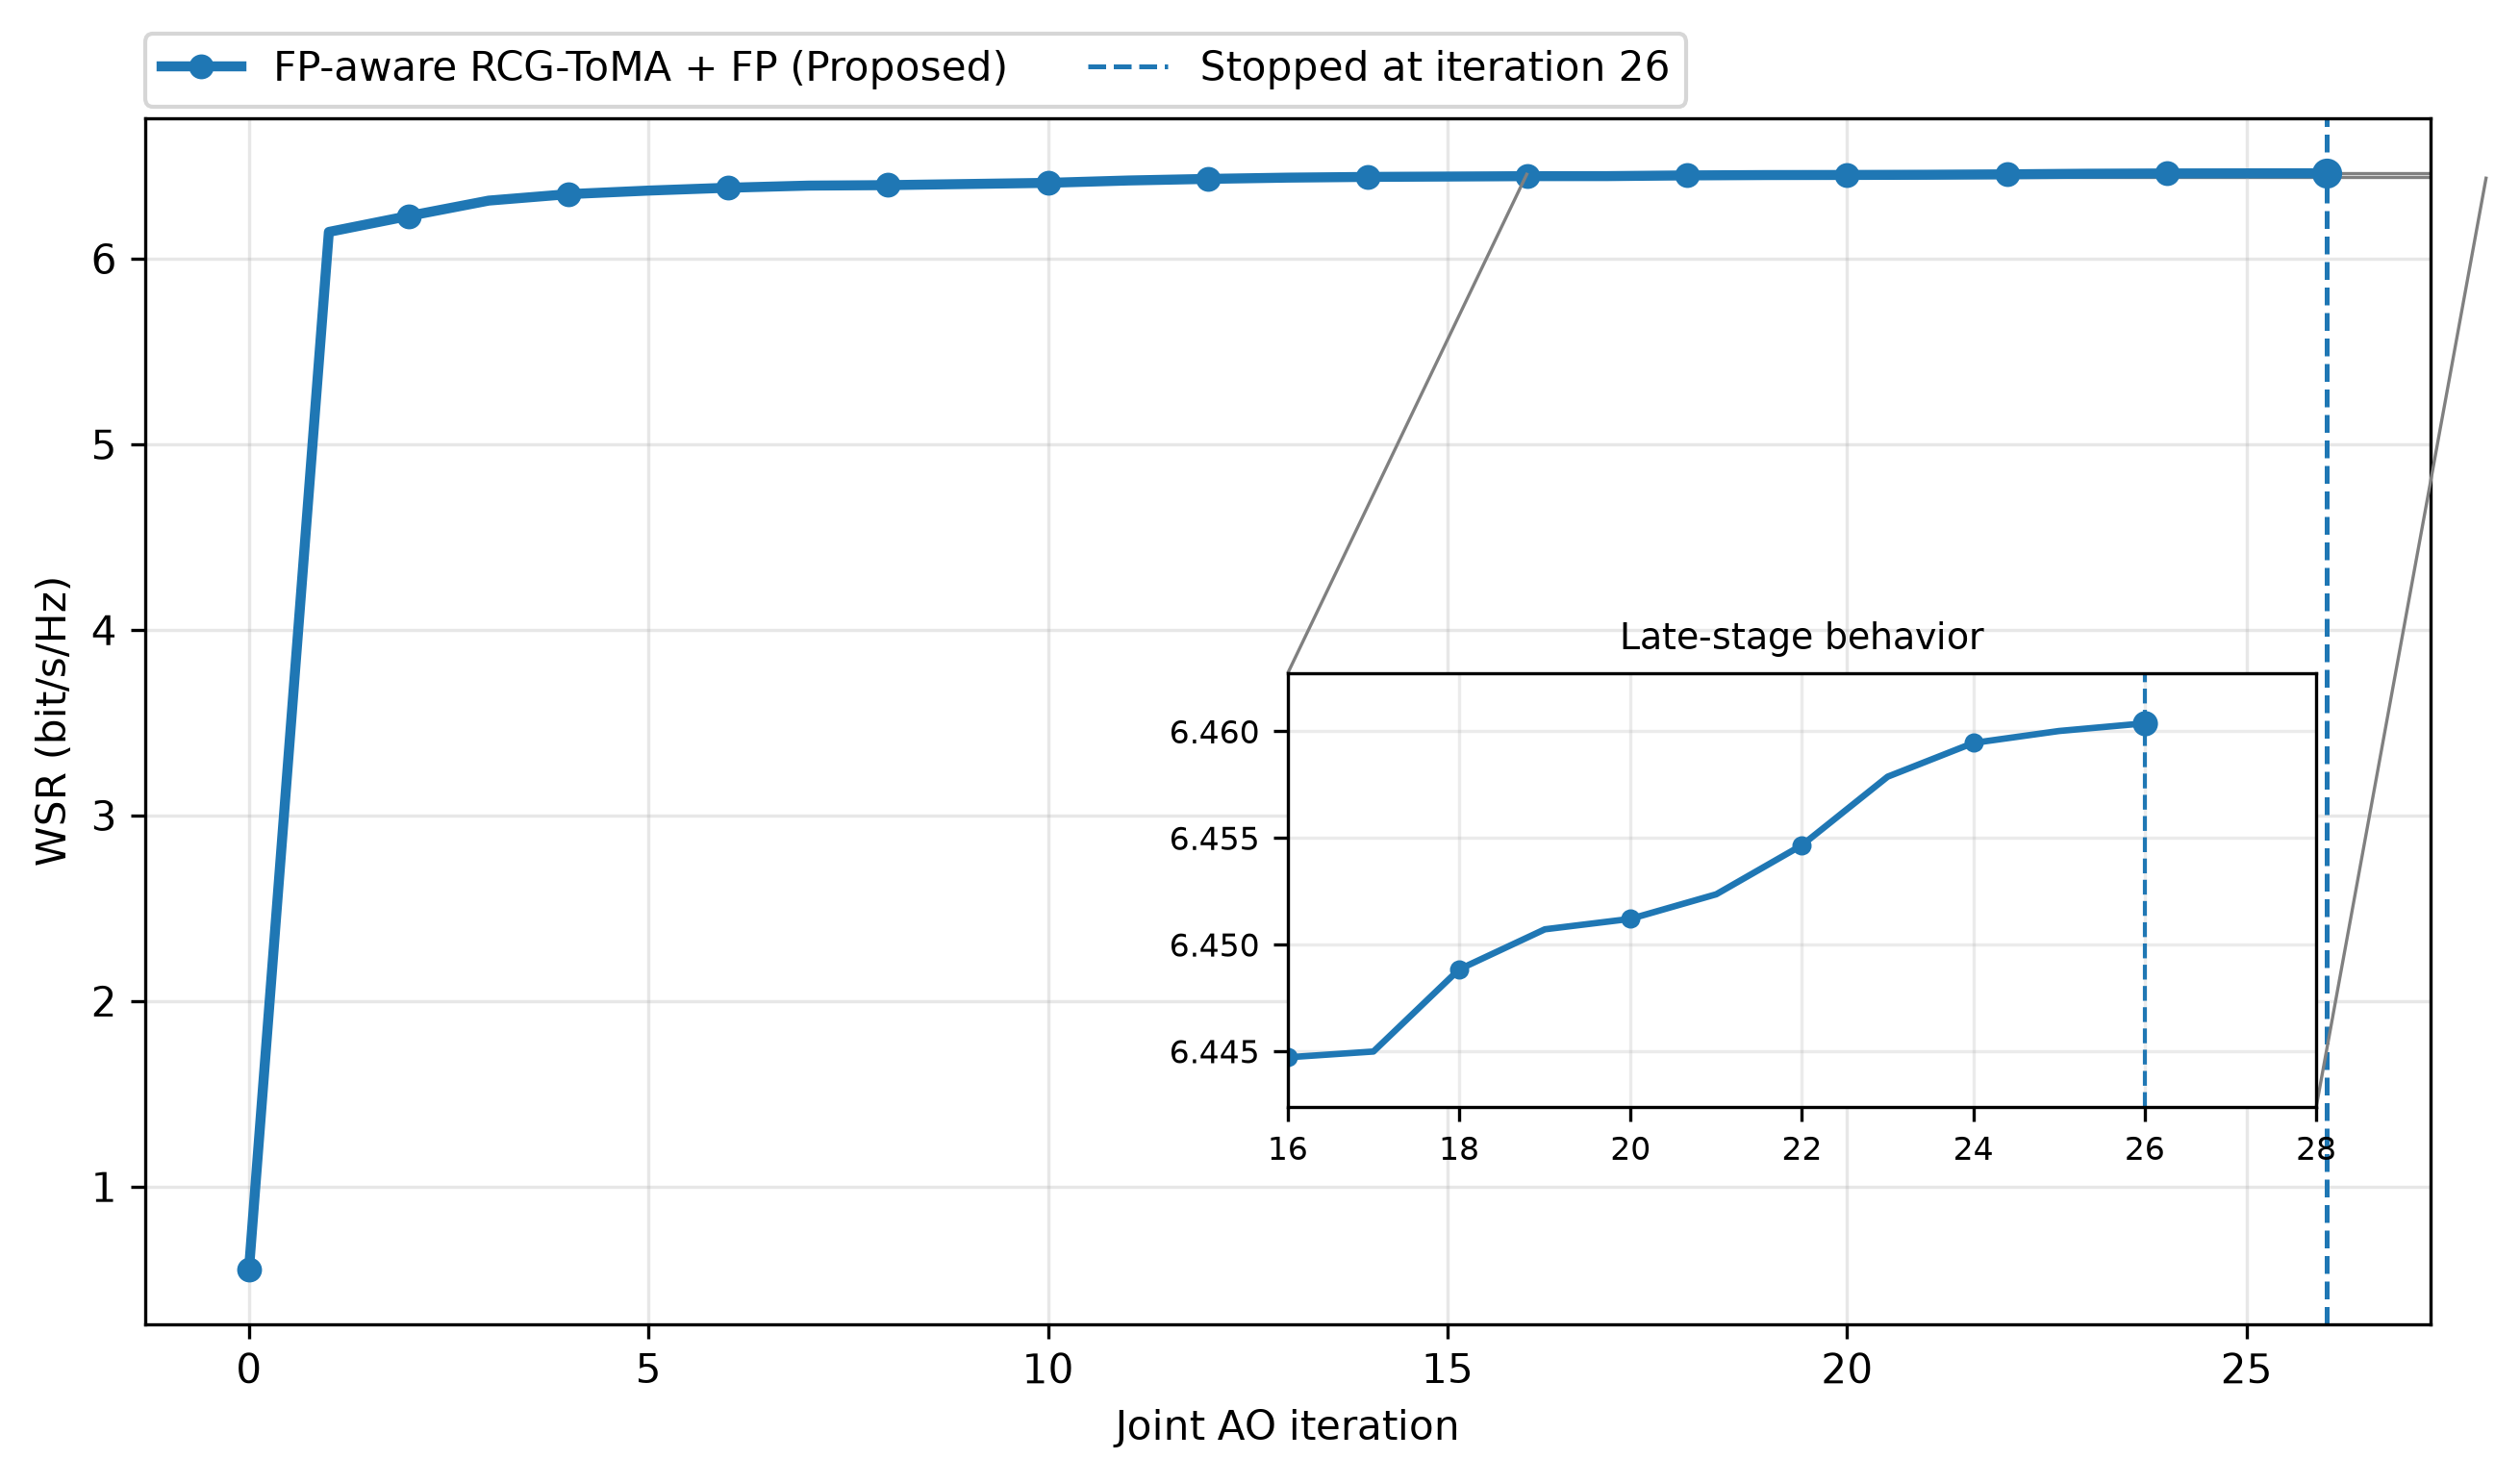
\includegraphics[width=\columnwidth]{figures/fig_convergence.png}
    \caption{Convergence behavior of the proposed FP-aware RCG-ToMA + FP
    algorithm in a representative random realization.}
    \label{fig:convergence}
\end{figure}

Fig.~\ref{fig:convergence} illustrates the convergence behavior of the
proposed FP-aware RCG-ToMA + FP algorithm in a representative random
realization. The WSR increases rapidly during the initial joint AO
iterations, rising from approximately $0.55$ bit/s/Hz to more than
$6.1$ bit/s/Hz after the first iteration. This substantial improvement
indicates that the joint adaptation of communication--sensing resources
and ToMA geometry can effectively enhance the initial system
configuration.

As the iterations proceed, the WSR continues to improve at a gradually
decreasing rate. The enlarged late-stage region shows that small
performance gains are still obtained during the later iterations, while
the variation in WSR becomes progressively smaller. The algorithm
terminates at the 26th joint AO iteration with a final WSR of
approximately $6.460$ bit/s/Hz.

These results demonstrate the numerical convergence behavior of the
proposed joint optimization method under the considered simulation
setting. However, since the original optimization problem is nonconvex,
the observed convergence does not guarantee global optimality.

% ============================================================
% C. Maximum DL Transmit Power
% ============================================================
\subsection{Impact of the Maximum DL Transmit Power}
\label{subsec:pdl}

\begin{figure}[!t]
    \centering
    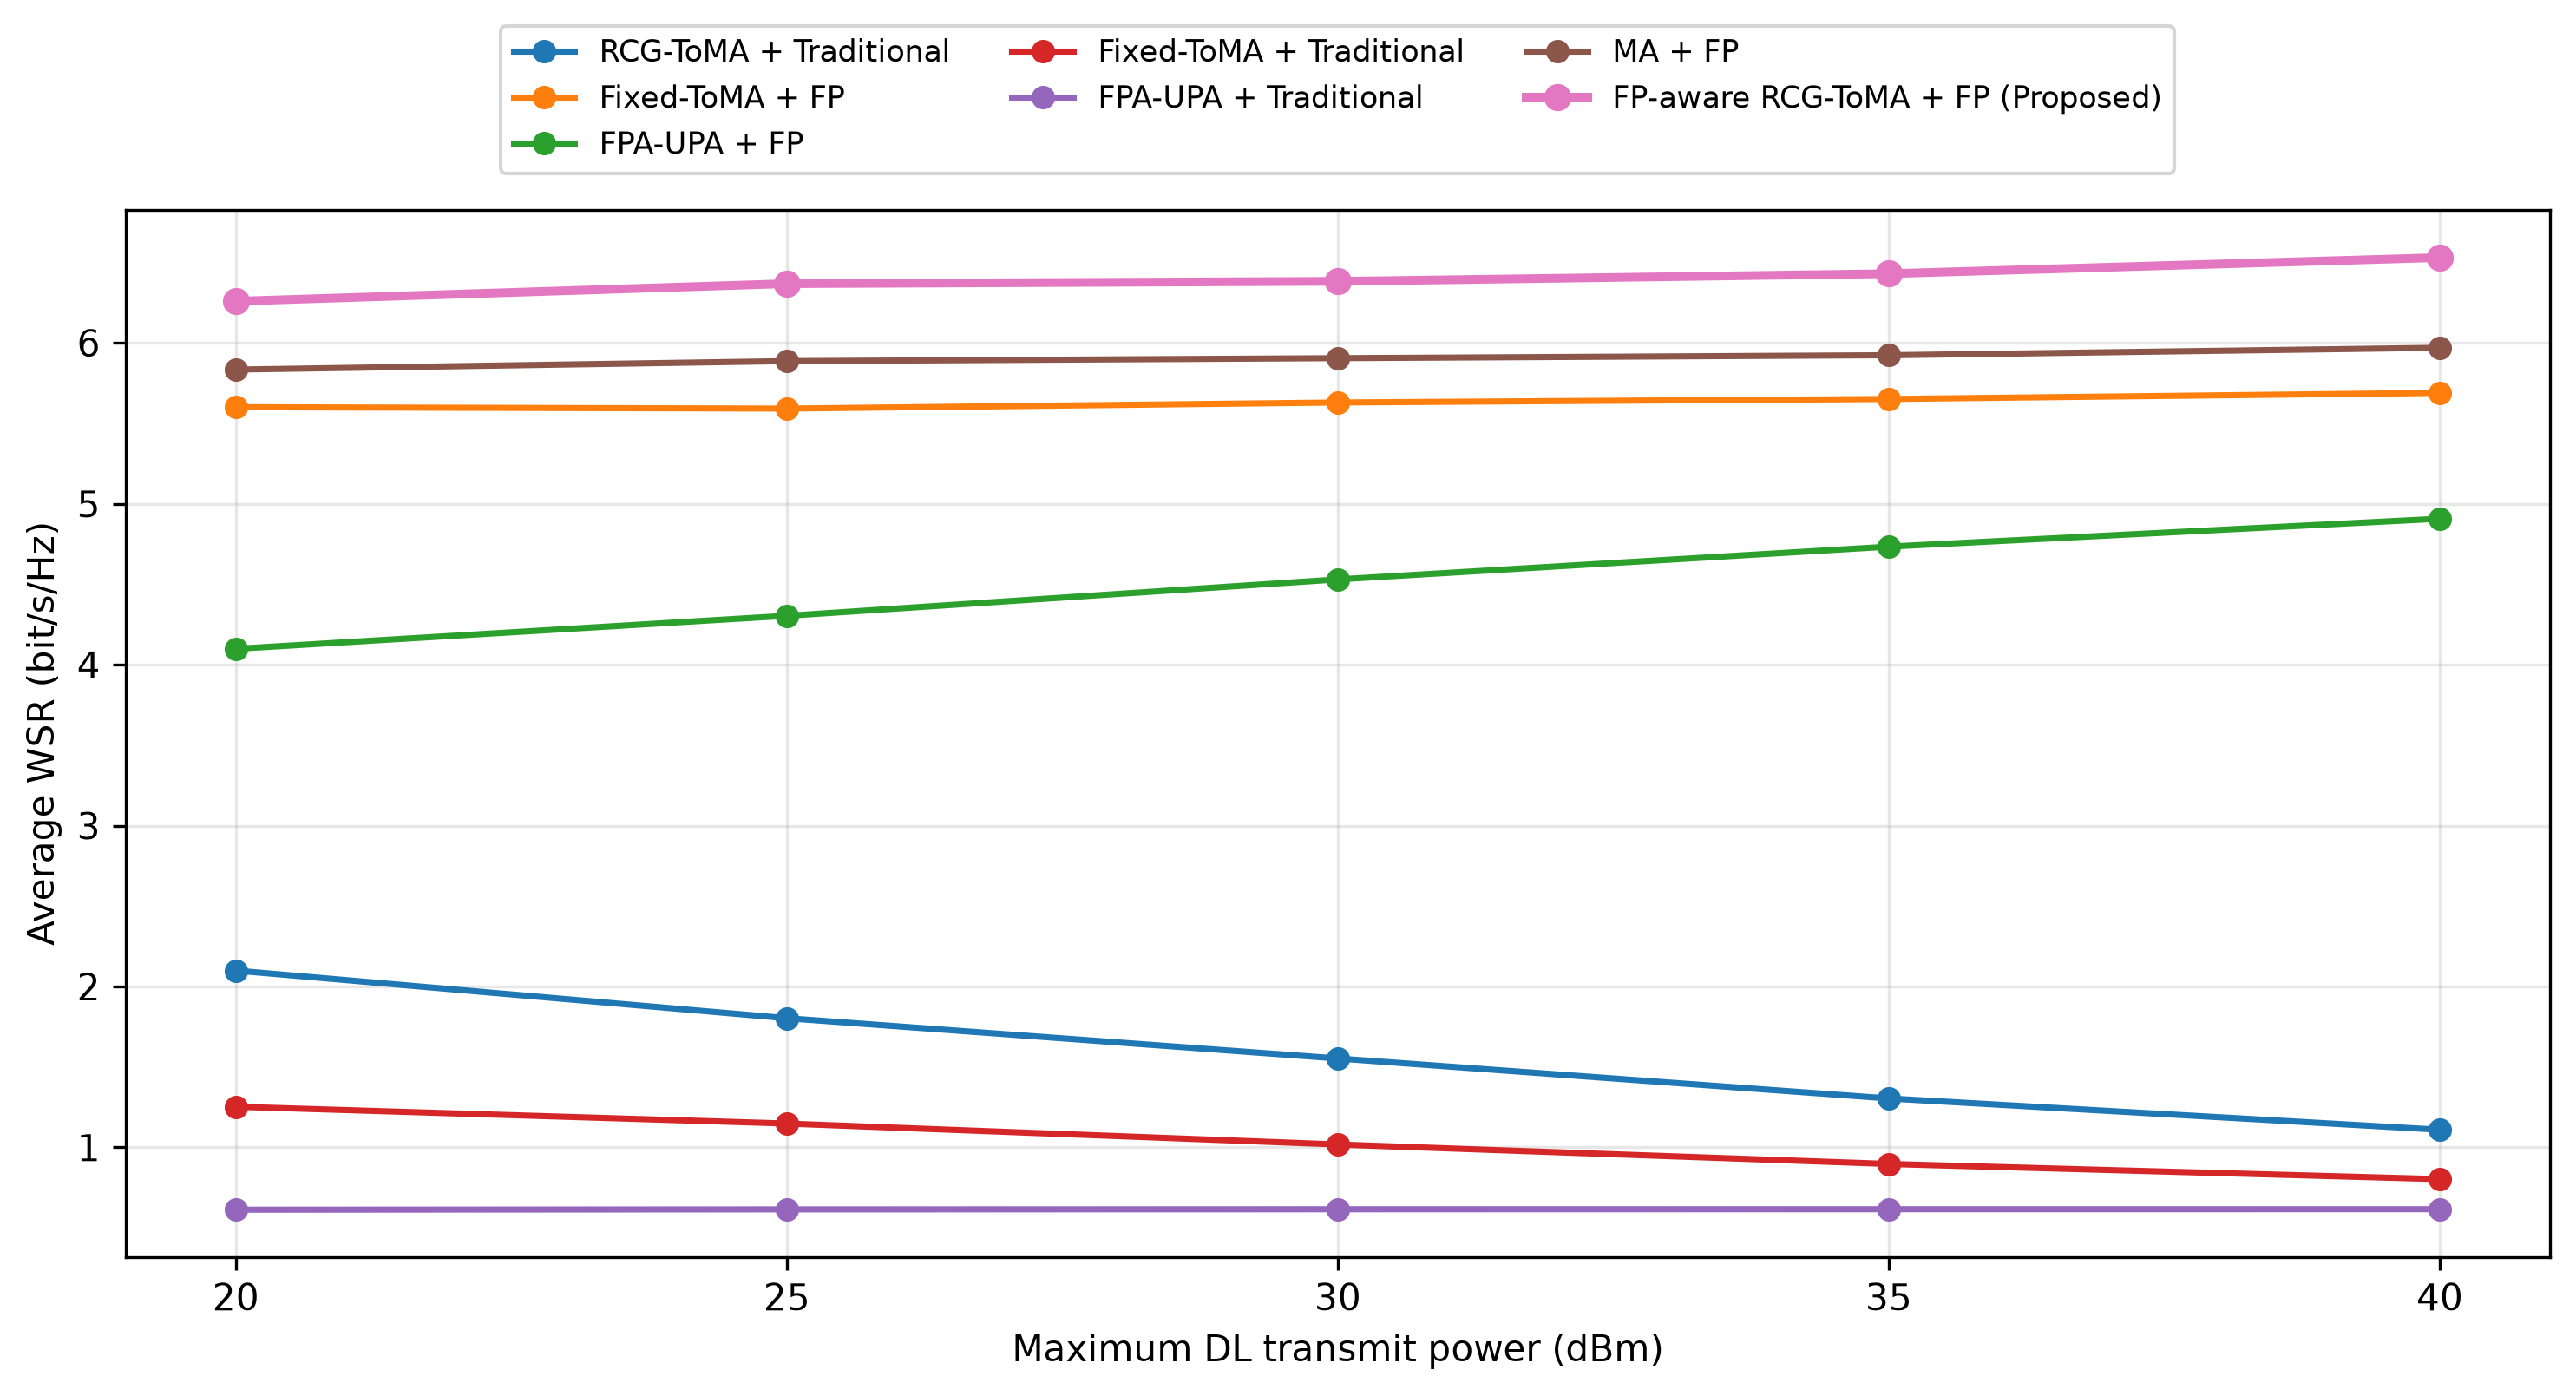
\includegraphics[width=\columnwidth]{figures/fig_pdl.png}
    \caption{Average WSR versus the maximum DL transmit power
    $P_{\rm D}^{\max}$.}
    \label{fig:pdl}
\end{figure}

Fig.~\ref{fig:pdl} shows the average WSR of different schemes versus the
maximum DL transmit power $P_{\rm D}^{\max}$. As
$P_{\rm D}^{\max}$ increases from $20$ dBm to $40$ dBm, the FP-based
schemes generally achieve improved or nearly stable WSR performance. In
particular, FPA-UPA + FP exhibits a relatively noticeable improvement,
while the proposed method, MA + FP, and Fixed-ToMA + FP show more
moderate gains.

In contrast, RCG-ToMA + Traditional and Fixed-ToMA + Traditional exhibit
decreasing WSR trends, whereas FPA-UPA + Traditional remains almost
unchanged. These results indicate that the implemented traditional
beamforming and resource-allocation strategies do not necessarily
exploit an increased transmit-power budget effectively. In the
considered full-duplex ISAC system, additional transmission power may
also affect the interference experienced by the UL communication and
sensing receivers. Therefore, the observed performance of these
traditional benchmark strategies should not be interpreted as the
globally optimal WSR under the corresponding power constraints.

The proposed FP-aware RCG-ToMA + FP method consistently achieves the
highest average WSR over the entire investigated transmit-power range,
followed by MA + FP. This demonstrates that the coupled movement of
antenna elements along ToMA cables can still provide effective spatial
reconfiguration capabilities when combined with joint
communication--sensing resource optimization.

Furthermore, the proposed method outperforms Fixed-ToMA + FP,
illustrating the performance benefit associated with optimizing the ToMA
geometry. Meanwhile, Fixed-ToMA + FP and FPA-UPA + FP outperform their
corresponding traditional-resource counterparts, respectively. Since
each comparison pair employs the same antenna architecture, these
results support the effectiveness of FP-based communication--sensing
resource allocation.

% ============================================================
% D. Residual Self-Interference
% ============================================================
\subsection{Impact of Residual Self-Interference}
\label{subsec:rsi}

Fig.~\ref{fig:rsi} shows the average WSR of different schemes versus the
residual-SI level.

\begin{figure}[!t]
    \centering
    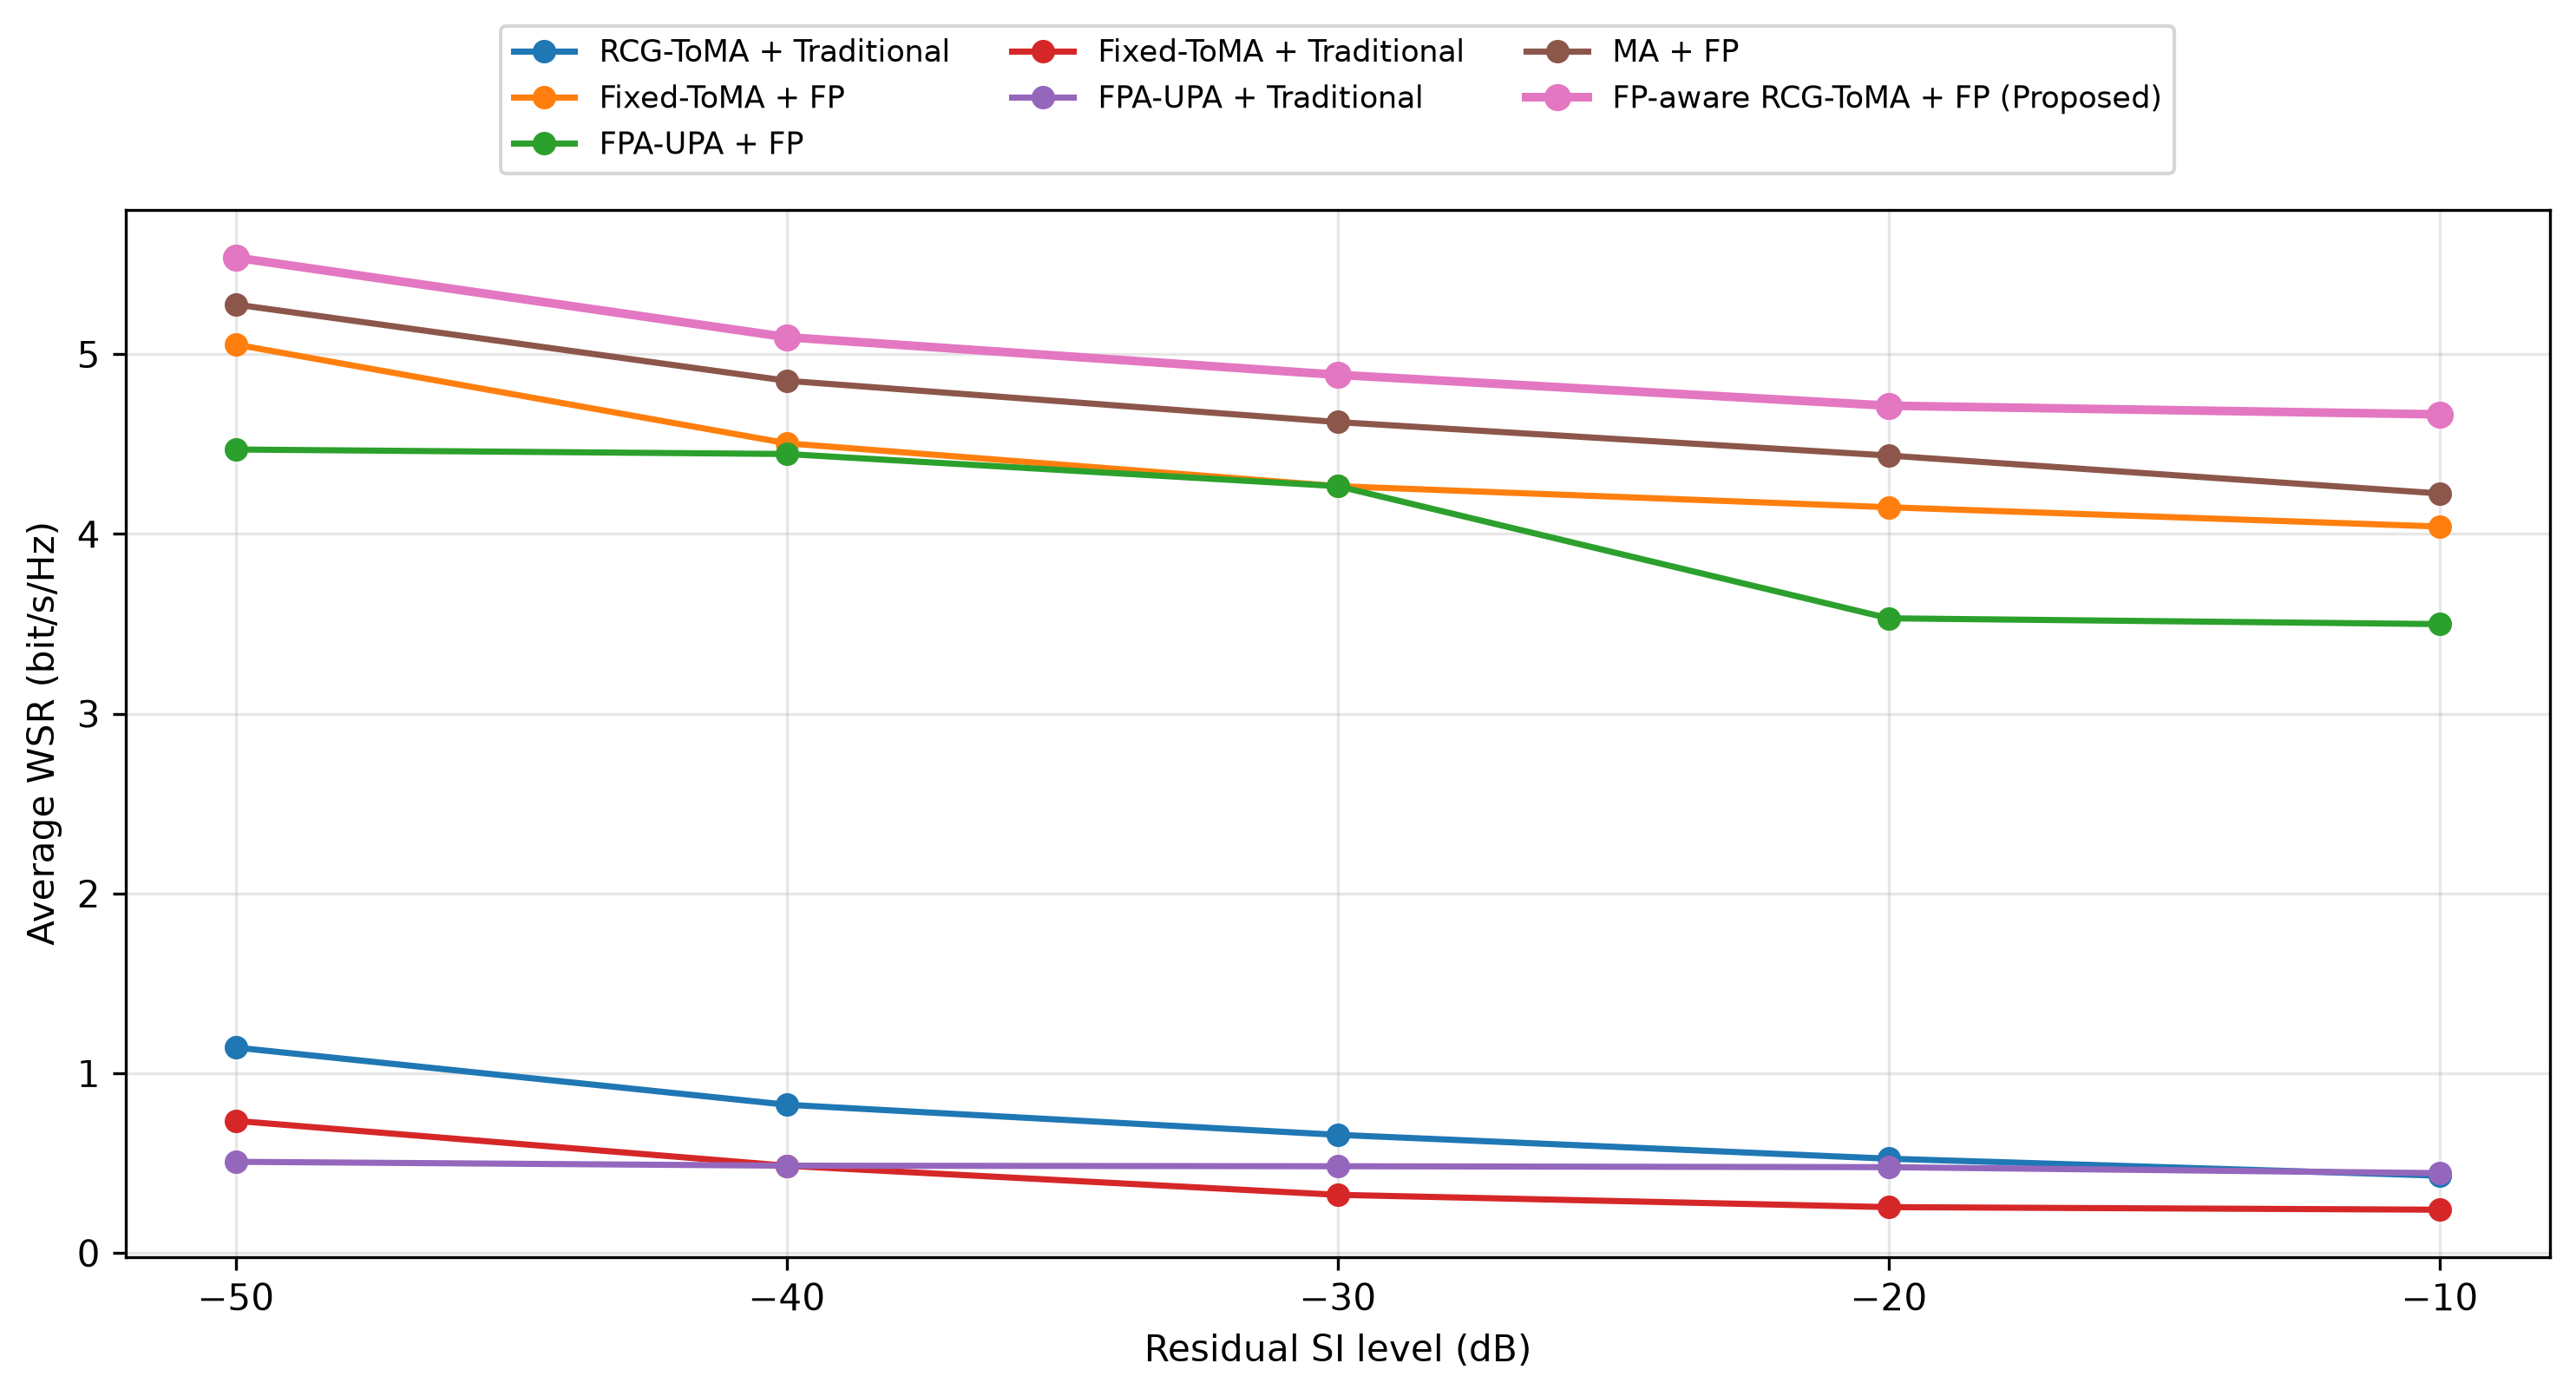
\includegraphics[width=\columnwidth]{figures/fig_rsi.png}
    \caption{Average WSR versus the residual-SI level
    $10\log_{10}(\rho_{\rm SI})$.}
    \label{fig:rsi}
\end{figure}

To investigate the sensitivity of the system performance to
residual self-interference (SI), the residual-SI level
$10\log_{10}(\rho_{\rm SI})$ is varied from $-50$ dB to
$-10$ dB. This range is considered for the residual-SI
sensitivity analysis, whereas the nominal residual-SI level
remains $-100$ dB, as specified in
Table~\ref{tab:simulation_parameters}.

As shown in Fig.~\ref{fig:rsi}, the average WSR of the
considered schemes generally decreases as the residual-SI
level increases. This behavior is consistent with the adopted
full-duplex ISAC model, where a larger $\rho_{\rm SI}$
increases the residual interference experienced by the main
UAV receiver. Since residual SI contributes to the
interference covariance matrices of both the UL communication
and sensing links, stronger residual SI reduces their
achievable SINRs for fixed transmission and reception
strategies, thereby limiting the overall WSR performance.

The proposed FP-aware RCG-ToMA + FP method consistently
achieves the highest average WSR across the entire
investigated residual-SI range, followed by MA + FP.
Although the WSR of both schemes decreases as residual SI
becomes stronger, the proposed method maintains a clear
performance advantage over MA + FP. This result demonstrates
the effectiveness of jointly optimizing the ToMA geometry
and communication--sensing resources under the considered
residual-SI conditions.

Furthermore, the FP-based schemes generally outperform
their corresponding traditional-resource benchmarks.
In particular, the performance improvement of
Fixed-ToMA + FP over Fixed-ToMA + Traditional and that
of FPA-UPA + FP over FPA-UPA + Traditional highlight
the importance of resource optimization in full-duplex
ISAC systems. These observations indicate that combining
antenna geometry optimization with FP-based resource
allocation provides effective performance improvements
across different residual-SI levels.

% ============================================================
% E. System Load
% ============================================================
\subsection{Impact of System Load}
\label{subsec:system_load}

Fig.~\ref{fig:load} investigates the average WSR under different system
loads by simultaneously varying the numbers of DL users, UL users, and
sensing targets, where $K=J=L$.

\begin{figure}[!t]
    \centering
    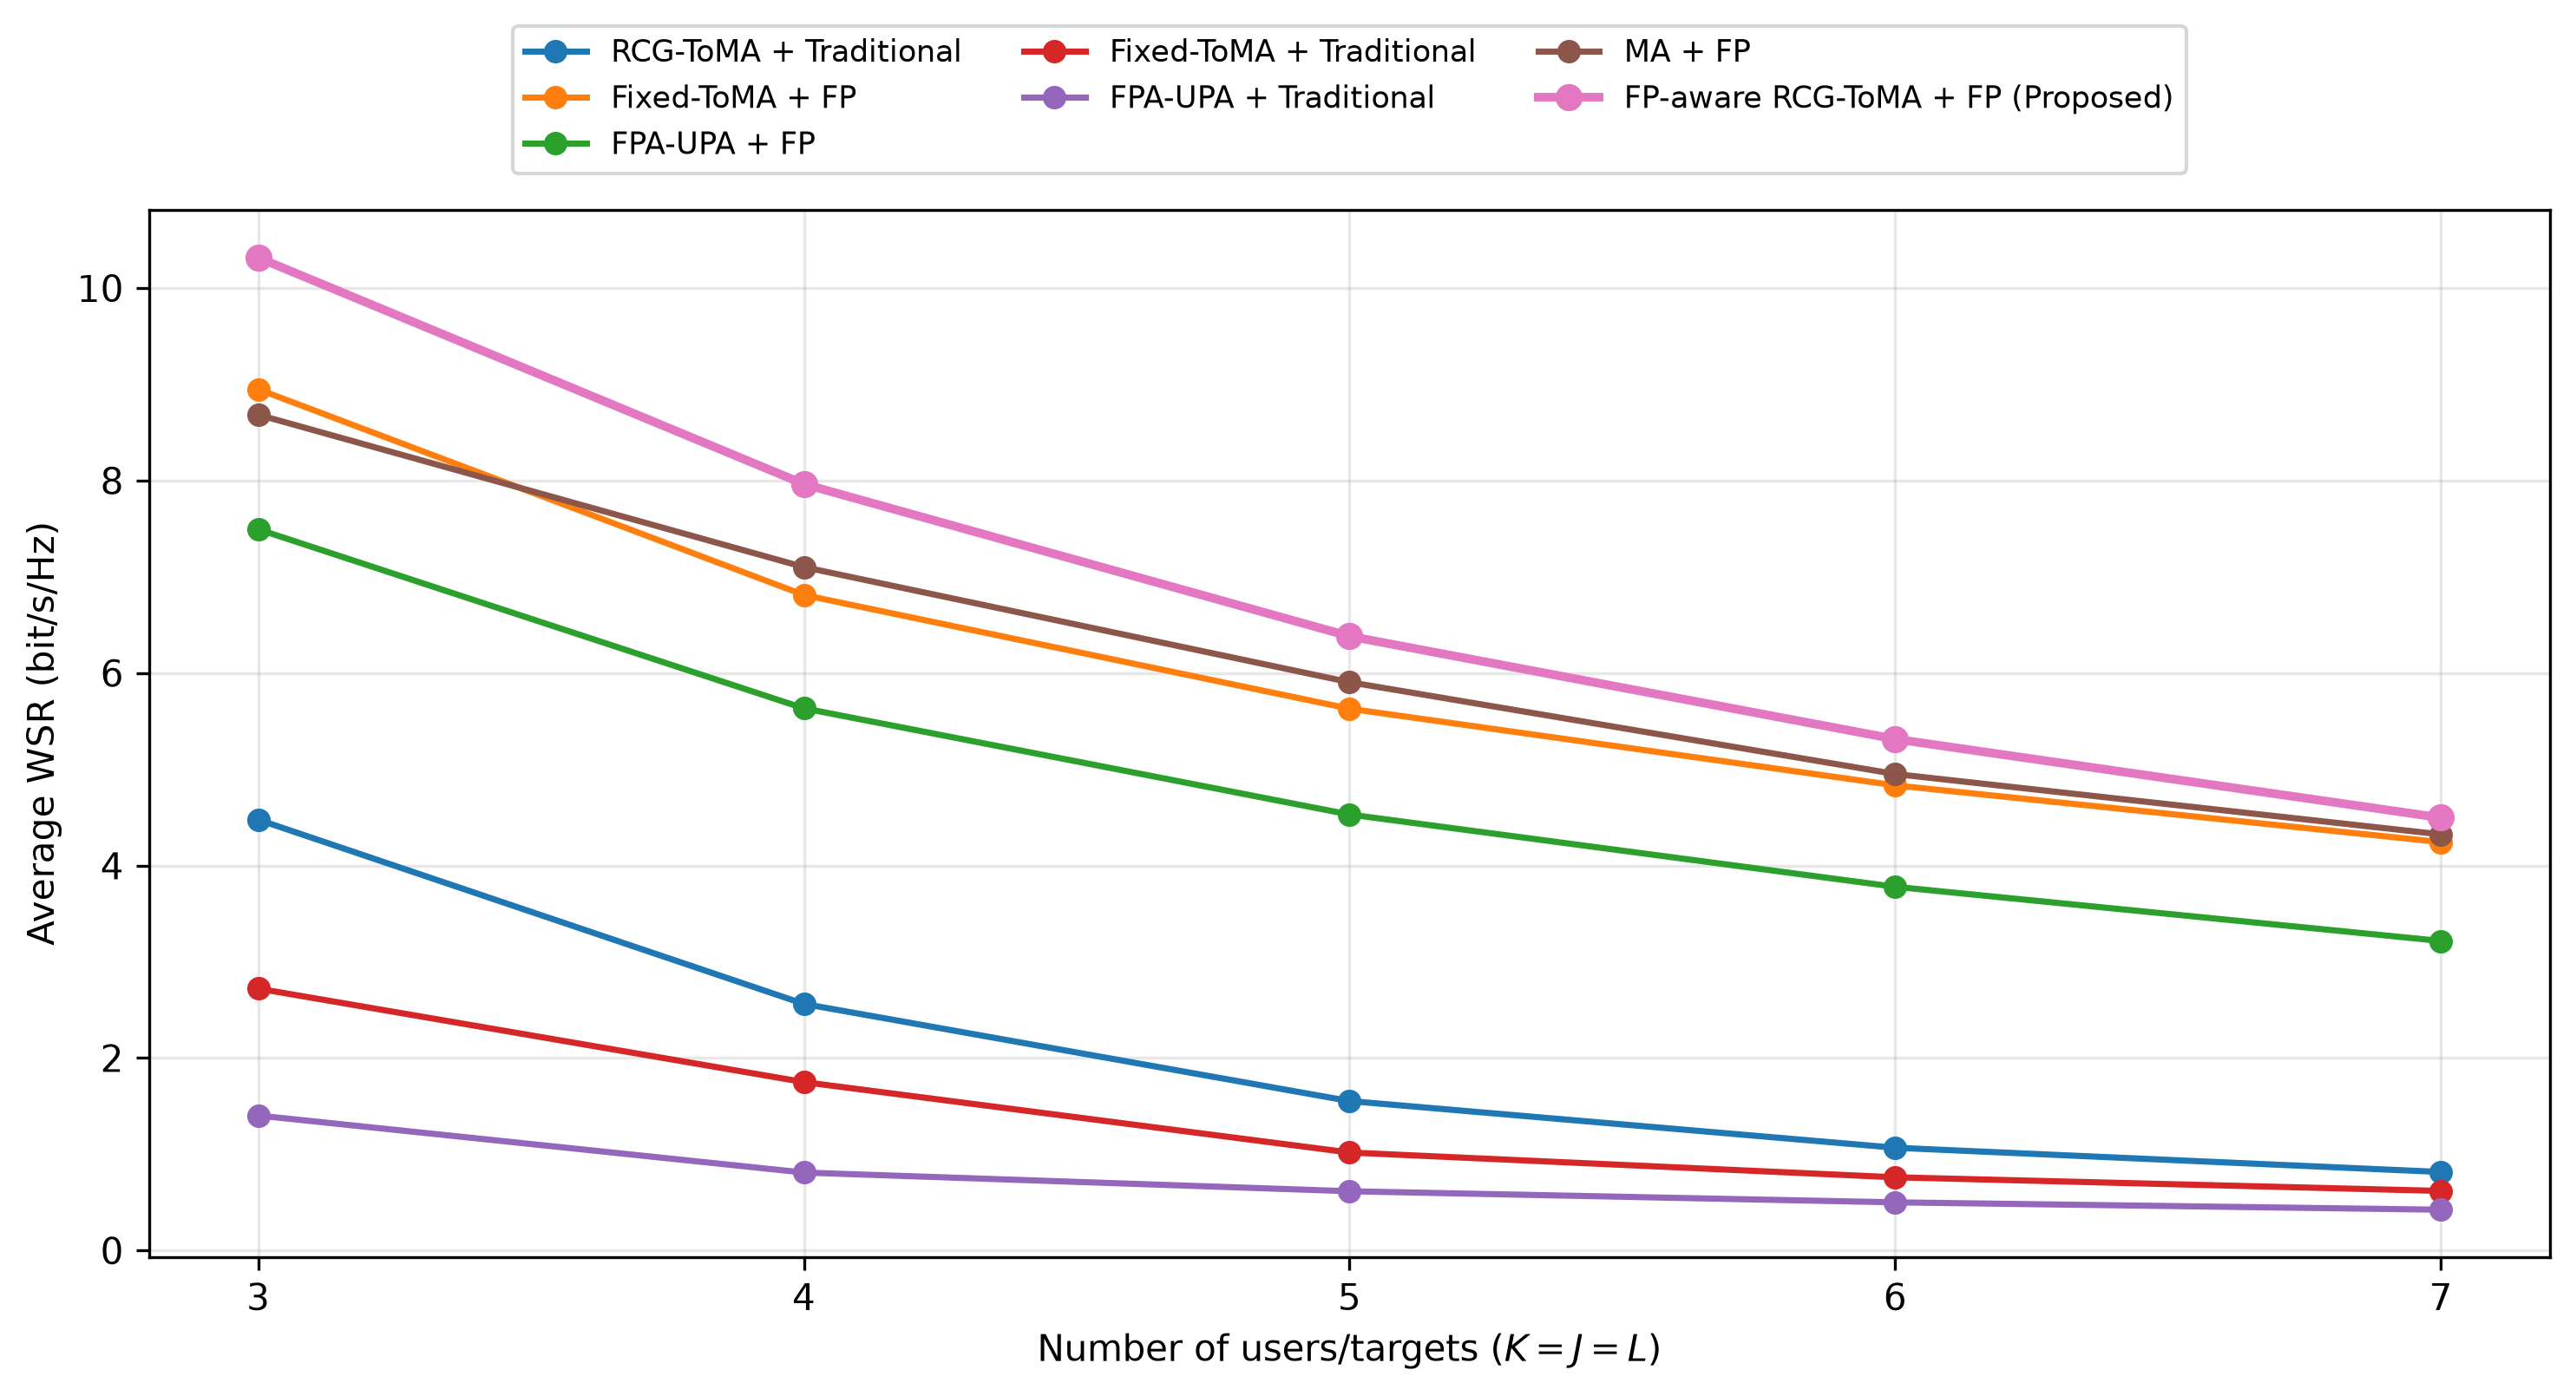
\includegraphics[width=\columnwidth]{figures/fig_load.png}
    \caption{Average WSR versus the system load, where $K=J=L$.}
    \label{fig:load}
\end{figure}

It can be observed that the average WSR of all schemes decreases as
$K=J=L$ increases from $3$ to $7$. This degradation is mainly caused by
two factors. First, the available transmit power, antenna elements, and
spatial degrees of freedom remain limited, while an increasing number
of communication users and sensing targets must share these resources.
Second, increasing the system load intensifies multiuser interference,
inter-target echo interference, and competition between communication
and sensing tasks.

Despite the increasing system load, the proposed FP-aware RCG-ToMA + FP
method maintains the highest average WSR over the entire considered
range. MA + FP achieves the second-best performance, while Fixed-ToMA +
FP and FPA-UPA + FP exhibit further performance degradation. These
results demonstrate that the joint optimization of ToMA geometry and
communication--sensing resources can more effectively exploit the
available spatial and power-domain degrees of freedom when the system
needs to simultaneously serve multiple communication users and sensing
targets.

The schemes employing traditional resource allocation experience more
pronounced performance degradation as the system load increases, with
FPA-UPA + Traditional exhibiting the lowest overall performance. This
further confirms that joint resource optimization becomes increasingly
important in heavily loaded multiuser and multitarget ISAC systems.

It should be emphasized that the horizontal axis in
Fig.~\ref{fig:load} represents $K=J=L$, rather than
$K=J=L=R_{\rm S}$.

The WSR is evaluated using normalized communication and sensing weights,
with every active DL user, UL user, and sensing target assigned the
weight $1/(K+J+L)$. Consequently, the decrease in WSR as the system load
increases reflects the change in normalized weighted performance and
should not be directly interpreted as a decrease in the unweighted
aggregate sum rate of all communication users and sensing targets.

\subsection{Communication--Sensing Trade-off Performance}
\label{subsec:tradeoff}

To evaluate the communication--sensing trade-off under different antenna
architectures, Fig.~\ref{fig:tradeoff} plots the sum communication rate
against the sum sensing rate achieved by four FP-based schemes. The two
performance measures are defined as
\begin{equation}
\begin{aligned}
R_{\rm C} &= \sum_{k\in\mathcal K} R_k^{\rm D}
          + \sum_{j\in\mathcal J} R_j^{\rm U}, \\
R_{\rm S} &= \sum_{l\in\mathcal L} R_l^{\rm S}.
\end{aligned}
\label{eq:tradeoff_sum_rates}
\end{equation}
For the considered setting with $K=J=L=5$, the group-weighted objective
is given by
\begin{equation}
F(\omega_{\rm C})=
\frac{\omega_{\rm C}}{10}R_{\rm C}
+\frac{1-\omega_{\rm C}}{5}R_{\rm S},
\label{eq:tradeoff_group_weight}
\end{equation}
where $\omega_{\rm C}\in[0.001,0.9]$ is evaluated at 20 specified
weight values. Each weight is optimized using independent cold-start
initializations, without transferring solutions between different
weights. Fixed-ToMA + FP, FPA-UPA + FP, MA + FP, and the proposed method
use 5, 1, 3, and 5 initializations, respectively. For each scheme and
weight, the converged candidate with the highest achieved WSR is
selected. All four schemes are evaluated under the same user and target
locations and common physical parameters, while employing their
respective antenna geometries and optimization procedures.
% ============================================================
% F.
% ============================================================
\begin{figure*}[!t]
\centering
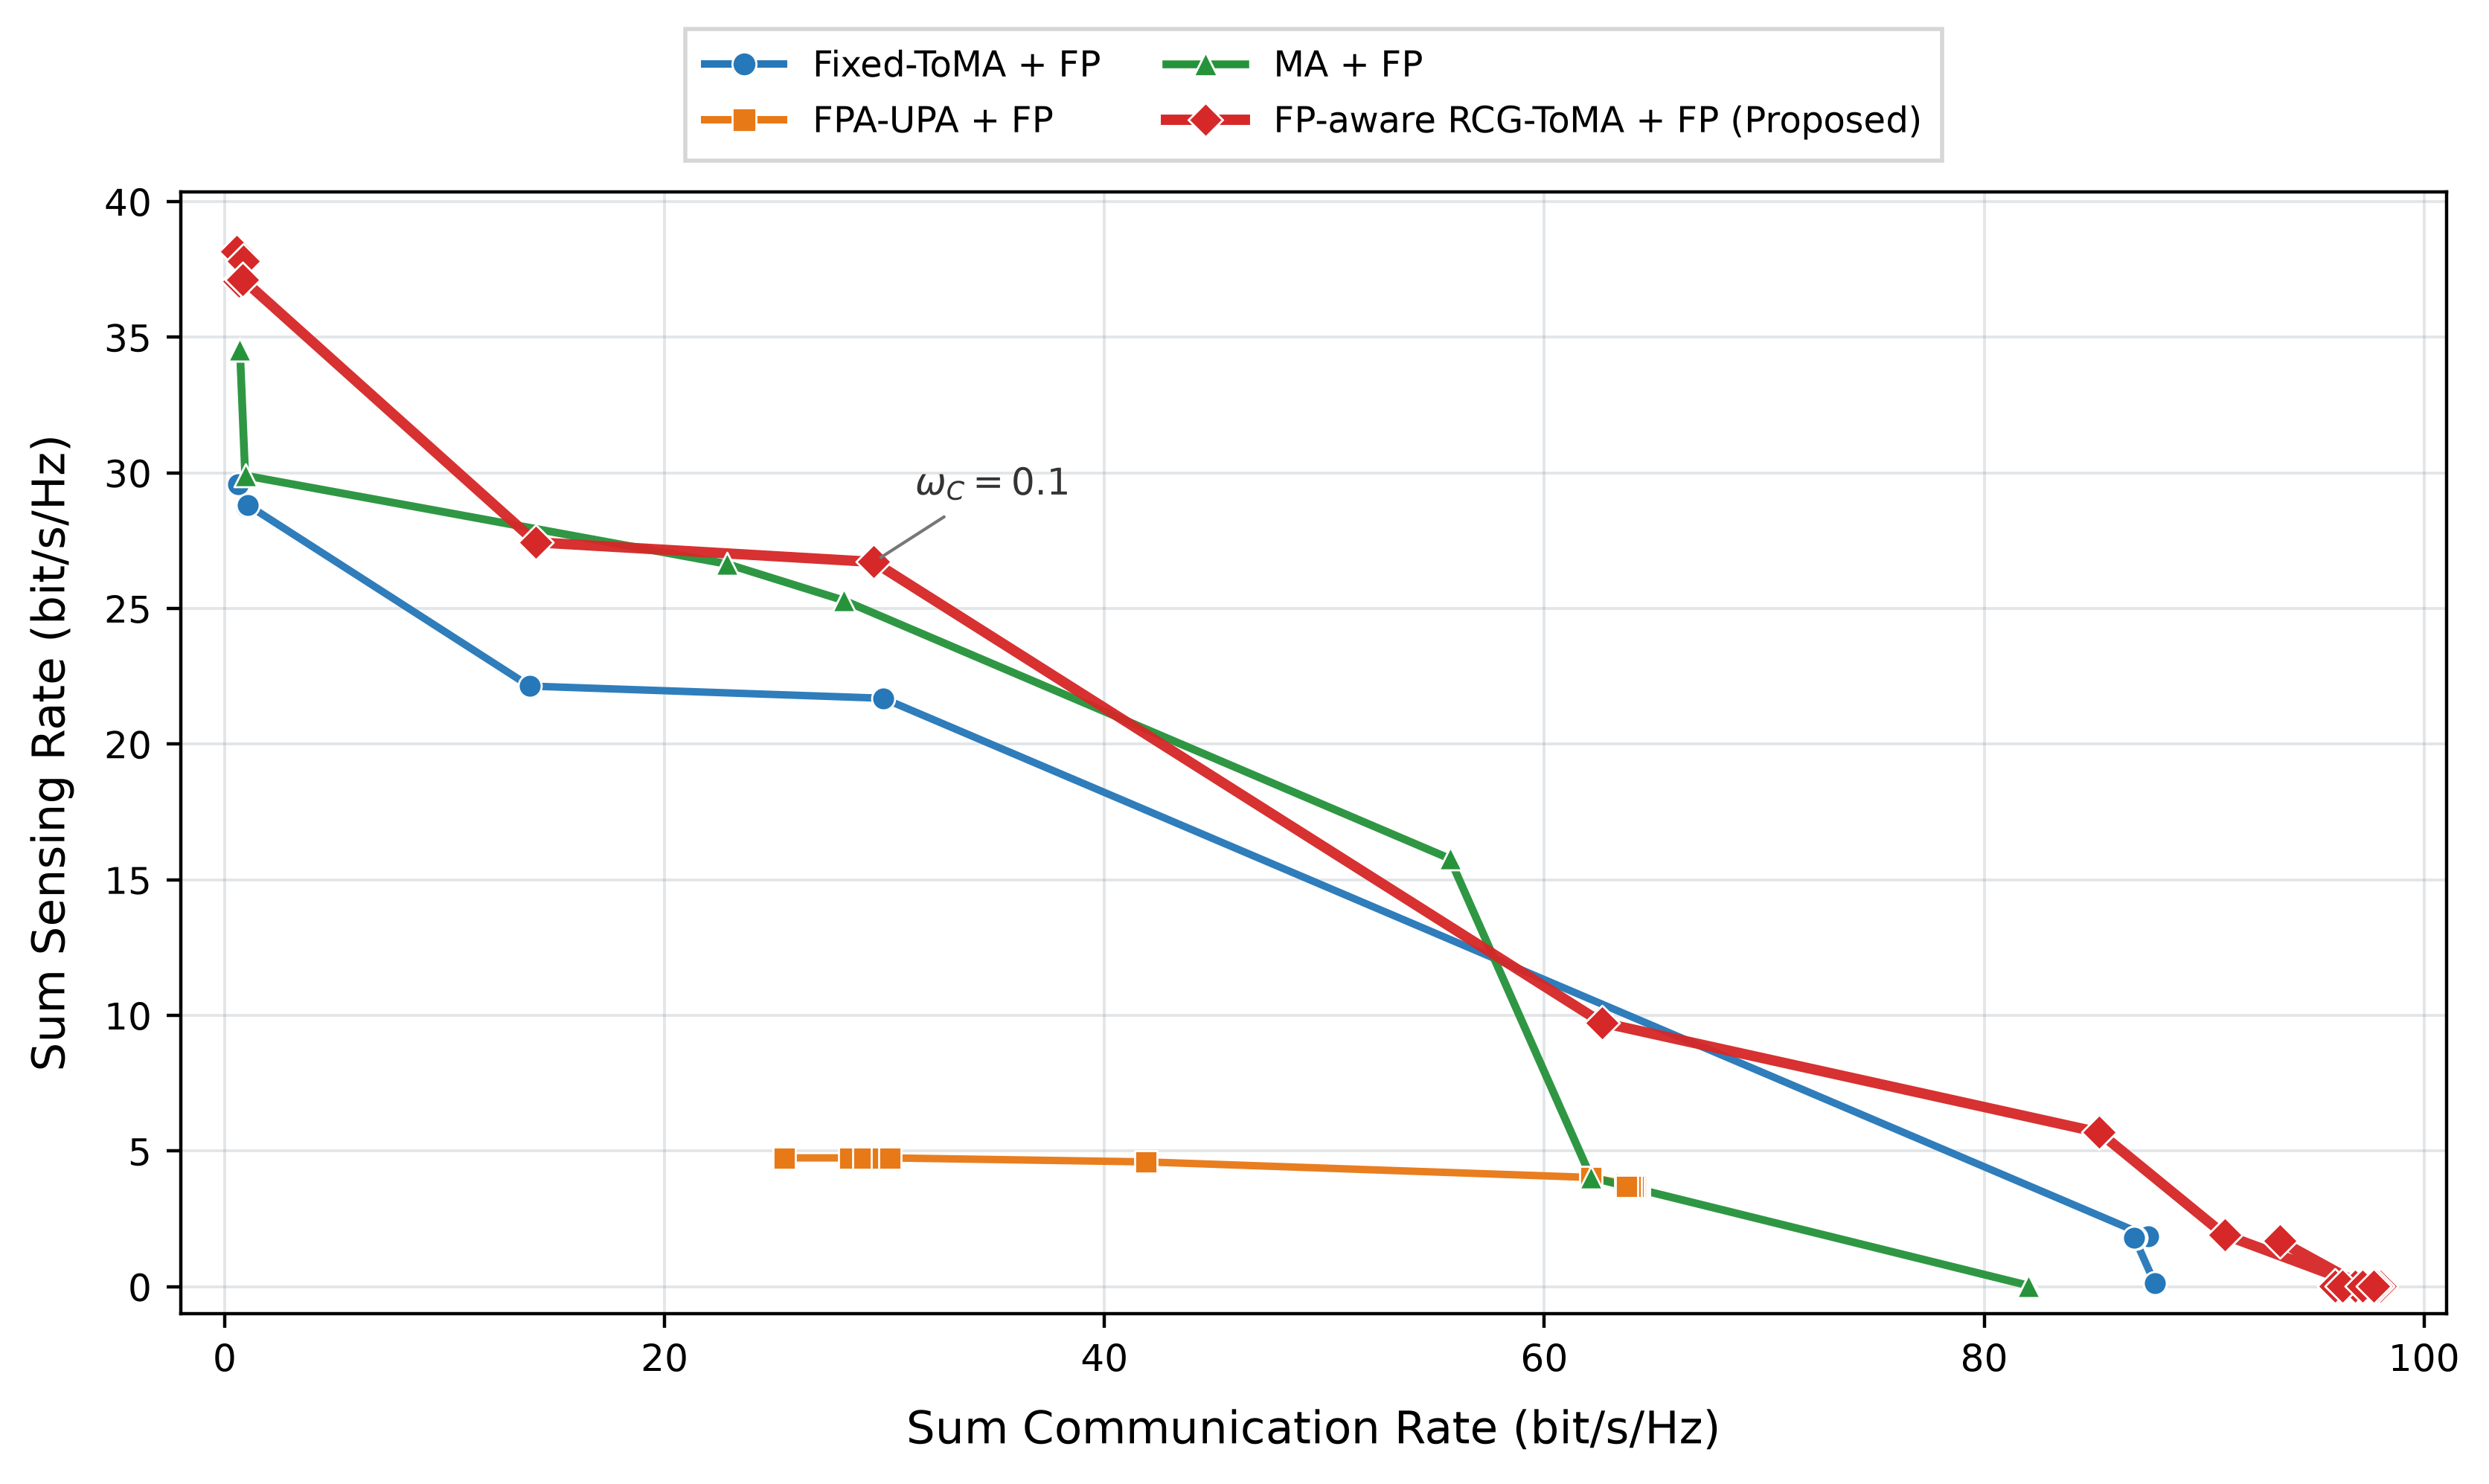
\includegraphics[width=0.92\textwidth]{figures/fig_tradeoff.png}
\caption{Communication--sensing trade-off achieved by different FP-based
schemes under independent cold-start initialization. Each marker is an
optimized operating point for one communication weight, and connecting
lines are provided only as visual guides.}
\label{fig:tradeoff}
\end{figure*}

As shown in Fig.~\ref{fig:tradeoff}, the obtained operating points
exhibit an overall trade-off: giving more weight to communication
generally increases $R_{\rm C}$ at the expense of $R_{\rm S}$. This
behavior reflects the coupling of transmit power, antenna spatial
degrees of freedom, UL power allocation, and communication--sensing
beamforming. The trend is not necessarily monotonic between every pair
of sampled weights because the underlying problem is nonconvex and each
weight is solved independently.

The proposed FP-aware RCG-ToMA + FP scheme achieves the highest WSR
among the four schemes at all 20 investigated weight values. Among its
sampled operating points, the maximum sum sensing rate is approximately
$38.15$ bit/s/Hz, while the maximum sum communication rate is
approximately $98.01$ bit/s/Hz; both maxima exceed the corresponding
sampled maxima of the benchmark schemes. At $\omega_{\rm C}=0.1$, the
proposed method achieves approximately
$(R_{\rm C},R_{\rm S})=(29.51,26.71)$ bit/s/Hz, illustrating an
operating point with appreciable communication and sensing performance.
These observations support the effectiveness of coupling ToMA geometry
reconfiguration with FP-based resource optimization under the
considered simulation conditions.

The benchmark schemes exhibit different achievable operating-point
patterns. MA + FP obtains competitive intermediate operating points,
whereas Fixed-ToMA + FP is limited by its fixed cable-array geometry.
FPA-UPA + FP attains relatively low sensing rates over its sampled
operating points. These differences may be associated with the distinct
geometric feasible regions, array responses, and position-optimization
procedures. In particular, independent element movement in MA and cable-coupled
movement in ToMA result in distinct geometric constraints, and their
feasible regions need not be nested.Hence, comparisons between
points having different communication rates should not be interpreted
as proof that one scheme universally dominates another at a fixed
communication rate.

Some sampled points display abrupt changes or slight non-monotonic
variations. Such behavior is consistent with independently initialized
numerical optimization of a nonconvex problem, potentially involving
different local solutions and resource-allocation regimes. Nevertheless,
the plots alone do not uniquely identify the cause of each transition.
Moreover, the connecting line segments do not imply that every
intermediate point has been obtained or is feasible. Since the sweep
does not include $\omega_{\rm C}=0$ or $1$, and global optimality is not
guaranteed, Fig.~\ref{fig:tradeoff} represents the achieved discrete
trade-off operating points rather than a globally optimal Pareto
frontier.

Overall, the proposed scheme achieves favorable communication--sensing
performance across the investigated weights and extends the range of
high-rate operating points observed in this experiment, despite the
coupled antenna-position constraints imposed by the ToMA architecture.

% 参考文献。
% 如果以后使用 references.bib，推荐采用下面两行。
% ============================================================
% \bibliographystyle{IEEEtran}
% \bibliography{references}

\begin{thebibliography}{1}
\bibitem{mathworks_radar_equation}
MathWorks, \emph{Radar Equation}, Radar Toolbox Documentation.
Accessed: Oct. 10, 2026. [Online]. Available:
\url{https://www.mathworks.com/help/radar/ug/radar-equation.html}
\end{thebibliography}

\end{document}
